% MANUSCRIPT.tex, the manuscript skeleton for the entry-contest paper (JITE).
% Created 6 October 2026 as pass 1 of the plan in TODO.md (item PLAN).
%
% PURPOSE
%   The manuscript. Four tables carry the body (introduction, model,
%   literature, conclusions), and the appendices carry every proof and the
%   content PROOFS.tex used to hold. PROOFS.tex was retired at pass 6
%   (7 October 2026). RETIREMENT.md records where each part of it went, and
%   checks/verify_retirement.py checks that record against the file in git.
%
% STRUCTURE THE CHECKER RELIES ON (checks/verify_manuscript.py)
%   Rows are written only through the four row macros below, and proofs only
%   through the mproof environment. IDs are K1, K2, ... (introduction),
%   M1, ... (model), L1, ... (literature) and C1, ... (conclusions).
%     \krow{ID}{headline}{model rows}{scope note}
%     \mrow{ID}{claim in words}{statement in symbols}{Lean theorems}
%     \lrow{ID}{bib key}{what we rely on}{verbatim quote}{page}{model rows}
%     \crow{ID}{statement}{model or literature rows}
%     \begin{mproof}{model row}{Lean theorems} ... \end{mproof}
%   Lists of rows or theorems are comma-separated. Lean theorem names are the
%   fully qualified names declared in lean/EntryContest.lean or under
%   lean/mathlib/.
%
% RULES THE CHECKER ENFORCES
%   Introduction rows point to model rows only. Conclusion rows point to model
%   or literature rows only. Every model row names Lean theorems that exist in
%   an audited Lean file and has exactly one proof in Appendix A naming the
%   same theorems. Every literature row's quote appears verbatim in the
%   paper's lit/ record. In every proof, plain English is at most 30% of the
%   text, measured as prose words over prose words plus mathematical tokens.

\documentclass[11pt]{article}
\usepackage[T1]{fontenc}
\usepackage[utf8]{inputenc}
\usepackage{mathptmx}
\usepackage{microtype}
\usepackage[a4paper,margin=1.8cm]{geometry}
\usepackage{amsmath,amssymb,amsthm}
\usepackage{booktabs}
\usepackage{array}
\usepackage{longtable}
\usepackage{graphicx}
\usepackage{url}
\usepackage[hidelinks]{hyperref}
\usepackage{natbib}

\emergencystretch=1.5em

\newcolumntype{P}[1]{>{\raggedright\arraybackslash}p{#1}}

\urlstyle{tt}
\makeatletter
\g@addto@macro\UrlBreaks{\do\.\do\_\do\,}
\makeatother
\newcommand{\lean}[1]{\path{#1}}
\newcommand{\rowref}[1]{#1}
\newcommand{\unv}[1]{\textit{Unverified:} #1}
\newcommand{\pend}[1]{\textit{Pending:} #1}

\newcommand{\krow}[4]{#1 & #2 & \rowref{#3} & #4 \\ \addlinespace}
\newcommand{\mrow}[4]{#1 & #2 & #3 & \lean{#4} & p.~\pageref{proof:#1} \\ \addlinespace}
\newcommand{\lrow}[6]{#1 & \citet{#2} & #3 & ``#4'' & #5 & \rowref{#6} \\ \addlinespace}
\newcommand{\crow}[3]{#1 & #2 & \rowref{#3} \\ \addlinespace}

\newenvironment{mproof}[2]
  {\subsection*{Proof of #1}\label{proof:#1}%
   {\raggedright\noindent\textit{Lean:} \lean{#2}.\par}\smallskip}
  {\par\hfill$\square$\par\medskip}

\title{Who Pays to Compete? Wealth, a Fixed Fee and Entry by Rank}
\author{Anurag Srivastava}
\date{Manuscript skeleton, 7 October 2026, revised 15 October 2026}

\begin{document}
\maketitle

\section{Introduction}

\subsection{Research question}
\label{sec:question}

A credential is often worth more as a token than as evidence of skill. An
institution that allocates scarce positions, and cannot cheaply observe the
quality it cares about, has reason to weight a standardised token that it can
verify at little cost: a credential is a cleaner status than the disorganised
status that comes from unverified providers. Once the token can be bought at a fixed price, who holds
it depends on who can afford it. Two current institutions show the pieces.
Chiba City allocates licensed daycare places, within priority tiers, to the
highest selection points, and adds four points for a family that uses an
unlicensed nursery or a babysitter for at least 64 hours a month; families
without such care still compete on their other points. Italian contracting authorities must award extra points in
public tenders to firms that hold a gender-equality certificate, which attests
a firm's employment policies against parameters set by decree; firms without
it still bid and can win. In the first the purchase is a service that earns
standing, and in the second the authority weights a certificate that attests
what it does not check itself. The sources are in
\path{lit/applications_2026}.

The question is what this interaction of credentialism and wealth produces on
its own. A fixed fee buys a component of standing in a contest for positions
awarded by rank; outsiders still compete on the base component, and wealth
matters only through the utility cost of the fee. How do the number who enter,
and the entrants' share of the positions, respond to the prize, the fee, a
spread of wealth, the number of challengers, and the weight the rule puts on
the base component? Accumulated skill and saving, the channels through which
wealth usually works, are absent by construction, so the answers isolate what
the purchasable token does. Why an institution chooses the weight is outside
the model, which takes it as given; the account above motivates the weight and is not derived here. Weberian closure, in which
outsiders cannot win, is the boundary at which the base component counts for
nothing. The model keeps apart the two things \citet{Weber1978} separates as
class and status. Wealth sets only the cost of entering, and the prize is won
by rank (rows L14 to L16 give the passages and where the parallel ends).

\subsection{Main answer}
\label{sec:answer}

The answer rests on the headline claims below, one lever at a time. Each is a
statement about the one-shot equilibrium at a given wealth profile and holder
of the position (Appendix~\ref{app:primitives}, ``The contest'').

\begin{itemize}
\item \textbf{The count and who enters.} Every pure-strategy equilibrium has the
  same number of entrants, and the richest of them entering is always an
  equilibrium (K1). Sorting by wealth needs only that the fee's utility cost
  falls with wealth, which strict concavity implies and which is weaker (K3).
\item \textbf{The prize and the fee.} A larger prize does not lower the count,
  a larger fee does not raise it (K5), and the prize caps entry for every number
  of challengers (K4).
\item \textbf{A spread of wealth.} A spread about a pivot moves the count in a
  direction set by one comparison, the marginal entrant against the pivot (K2).
  This sign rule is new among the papers read (C1, C5).
\item \textbf{The number of challengers.} As challengers are added, the first
  entrant's gain can rise and then fall, and never falls and then rises (K6).
\item \textbf{The weight on the base component.} A rule that weighs the base
  component more draws no more entrants (K8) and gives them no larger share of
  the prize (K7), a sign that is new among the papers read (C9, C12). It does
  not thereby pick a better winner. With the entrants fixed the winner's base
  component does not fall, but once entry responds a common bonus, such as
  Chiba City's four points, can leave the winner with a lower base component
  (K9).
\item \textbf{The entrants' share.} The share of the prize taken by the
  entrants is set by the count and does not fall as more enter; when entry buys
  nothing it is $\frac{k+1}{Q+1}$ with $k$ entrants (K7). As a function of the
  count it is new among the papers read (C13).
\end{itemize}

\subsection{Headline claims}
\label{sec:headlines}

\footnotesize
\begin{longtable}{@{}P{0.8cm}P{7.0cm}P{1.9cm}P{6.4cm}@{}}
\caption{Headline claims, each traced to the model rows it rests on.}\\
\toprule
\textbf{ID} & \textbf{Headline} & \textbf{Model rows} & \textbf{Scope note} \\
\midrule
\endfirsthead
\toprule
\textbf{ID} & \textbf{Headline} & \textbf{Model rows} & \textbf{Scope note} \\
\midrule
\endhead
\bottomrule
\endfoot
\krow{K1}{Every pure-strategy equilibrium, with an indifferent challenger
  entering, has the same number of entrants, $k^*$, and the $k^*$ richest
  challengers entering is always one of them.}
  {M5, M6, M7, M8, M26, M27, M29, M30}
  {The count is pinned. Who enters is pinned when the condition of M7 holds,
  and need not be otherwise. The count rests on a gain that depends on the
  number of entrants alone (M26); for some laws of the bought component that
  differ by identity, falling with wealth (M27) or rising with it (M29), and
  some costs,
  it is not pinned. An incumbent who competes under the same rule, taken to be
  the lowest-cost player, sits out while a challenger enters only when
  $g(k^*)<\kappa_0$ and $\kappa_{k^*}\le g(k^*-1)$ (M30). At exact ties, with
  an indifferent challenger staying out, other counts can occur.}
\krow{K2}{The effect of a pivot-spread of wealth on how many enter has a sign
  set by one comparison. Entry weakly rises when the marginal entrant stands at
  or above the pivot, and weakly falls when it stands at or below.}
  {M12, M13, M14, M15}
  {Proved for pivot-spreads (M13). For any change of profile, a two-rank
  comparison signs the change outside the band (M12, M14); inside the band the
  signs of the change settle nothing (M14), and the mean cannot replace the
  pivot (M13). A strict fall is shown only for linear spreads with a large
  enough stretch, when the fee's utility cost diverges at the fee (M15).}
\krow{K3}{Given score laws that do not depend on who enters, the sorting needs
  only that the fee's utility cost falls with wealth, which strict concavity
  implies and which is strictly weaker.}
  {M5, M8, M23, M24, M26}
  {No condition on $u'''$ is used. When the law of the bought component differs
  by identity the sorting can fail (M27). Wealth sorting into a tournament is in print, by
  example (Lazear and Rosen), under declining absolute risk aversion, which
  needs $u'''>0$, so the mechanism is not claimed as new. Hu, Immorlica and
  Vaughan derive a group cost condition the same way, the same outlay weighing
  more in the disadvantaged group's utility (L33).}
\krow{K4}{Entry is capped by the prize for every number of challengers. An
  index $m$ with $\kappa_m\le\Delta(m)$ has $(m+1)\kappa_m\le V$, and every
  member $i$ of an equilibrium $S$ has $|S|\,\kappa_i\le V$.}
  {M10}
  {The accounting behind the cap is in print for identical agents (Fu, Jiao
  and Lu; Fu and Lu). It replaces the old mobility ceiling and is not claimed
  as new.}
\krow{K5}{A larger prize does not lower the number of entrants, and a larger
  fee does not raise it.}
  {M11}
  {Weak monotonicity only.}
\krow{K6}{When the score gap is single-peaked, the first entrant's gain can
  rise and then fall in the number of challengers, and it never falls and then
  rises. With a uniform base component it never falls, for some base
  components it must eventually fall, and stochastic dominance alone does not
  sign it.}
  {M16, M17, M18, M19, M20, M21, M22}
  {The absence of an interior minimum is Ryvkin and Drugov's Karlin step
  applied to the gain, with the score gap in place of the noise density, and
  the message that no such prediction is universal is theirs (L8, C12). What
  is new among the papers read is the uniform case and, for a bought component
  of two values, a condition on the base component that makes the gap
  single-peaked (C7).}
\krow{K7}{The entrants take the prize with a probability that does not fall
  as more of them enter. With $k$ entrants it equals $\frac{k+1}{Q+1}$ when
  entry buys nothing, and, with costs fixed, it does not rise as the rule
  weighs the base component more.}
  {M28, M31}
  {The share counts positions and not their pay; earnings after entry are
  outside the model (Appendix~\ref{app:primitives}). Its direction in the
  weight on the base component is that of the count (K8). The entrants' share
  as a function of how many enter is new among the papers read (C13).}
\krow{K8}{With the fee, the prize and the wealth profile fixed, the number of
  entrants does not rise as the rule weighs the base component more, and
  neither does the gain from entering at any number of entrants.}
  {M28}
  {Proved with the incumbent scored as an entrant, for every atomless law of
  the base component, every law of a non-negative bought component and every
  number of challengers. For an incumbent protected from the rule, whose law
  does not move with the weight, the argument does not apply
  (Appendix~\ref{app:primitives}). The sign is weak, and its size is not
  derived. In the two noise-comparative entry models read the sign is the
  opposite, because effort rises with the accuracy of the ranking and competes
  away the rents of entry, while a fixed fee does not rise (C9). The sign is
  new among the papers read (C9, C12).}
\krow{K9}{With the entrants fixed, a rule that weighs the base component more
  never leaves the winner with a lower base component. Once entry responds it
  can, as with a common bonus.}
  {M32}
  {The first part holds pointwise, for any laws and any bought scores, for
  weights up to one. The second is shown by one example, with one challenger,
  a uniform base component and a common bonus; how large the fall can be and
  how often it occurs are not derived. A common bonus washes out when every
  player holds it and favours its holders once some stop buying (K8). The
  result is a scope on K8, not a claim of novelty.}
\end{longtable}
\normalsize

\section{The model in brief}
\label{sec:brief}

\paragraph{Summary.} One prize of fixed value $V$ goes to the highest score
among an incumbent and $Q$ challengers. Challengers differ in wealth, and every
challenger knows the whole wealth profile. Each challenger makes one choice,
whether to enter by paying a fee $c$ that is the same for all. A challenger's
score is $\sigma_i=\mu r_i+(1-\mu)s_ie_i$. The base component $r_i$ is drawn
for everyone, and the bought component $s_i\ge0$ counts only for an entrant
($e_i=1$). The rule's weight on the base component is $\mu$. An outsider still
competes, on the base component alone. Both components are drawn after the
choices, from laws that do not depend on wealth, so no challenger knows her own
score when choosing. The incumbent is scored as an entrant. A challenger enters
when the gain from entering, $\Delta(m)$ with $m$ other entrants, covers the
utility cost of the fee, $\kappa(w)=u(w)-u(w-c)$. The cost falls with wealth,
and the gain falls as more others enter. These two facts pin the number of
entrants, $k^*$, in every pure-strategy equilibrium, and the $k^*$ richest
entering is always an equilibrium.

\footnotesize
\begin{longtable}{@{}P{1.8cm}P{3.8cm}P{2.8cm}P{3.8cm}P{3.3cm}@{}}
\caption{The players, their choices and what each optimises.}\label{tab:players}\\
\toprule
\textbf{Player} & \textbf{Who it is} & \textbf{Choice} & \textbf{Objective} & \textbf{Known when choosing} \\
\midrule
\endfirsthead
\toprule
\textbf{Player} & \textbf{Who it is} & \textbf{Choice} & \textbf{Objective} & \textbf{Known when choosing} \\
\midrule
\endhead
\bottomrule
\endfoot
Challenger $i$ & One of $Q$, $i\in\{0,\dots,Q-1\}$, with wealth $w_i$, indexed
  from the richest. One with $w_i\le c$ does not enter. & Enter or not,
  $e_i\in\{0,1\}$. No effort and no amount to bid. & The one-period expected
  payoff $u(w_i-c\,e_i)+V\Pr(i\text{ wins})$, given the others' choices; a
  repeated contest is this game if players are myopic or value holding the
  position alike (Appendix~\ref{app:primitives}). & $V$, $c$,
  $\mu$, the laws of $r$ and $s$, the whole wealth profile. Not her own
  draws. \\ \addlinespace
Incumbent & The holder of the position, scored as an entrant ($C=F$). & None in
  M1 to M29, M31 and M32, where she always competes and holds the bought
  component; whether she paid for it enters no result, since her payoff does
  not. In M30, enter or not, paying $c$ like a challenger, as player $0$ with
  the lowest cost. & In M30, the same as a challenger's. & As a challenger. \\ \addlinespace
Nature & & Draws $r_i$ and $s_i$, independent of each other, across players
  and of wealth. & None. & \\ \addlinespace
The institution & Not a player. & Fixes $V$, $c$ and $\mu$, which the
  comparative statics move one at a time. & None in the model; why it chooses
  $\mu$ is outside the model. & \\
\end{longtable}
\normalsize

\paragraph{Entry, equilibrium and timing.} Entering changes a challenger's
expected payoff by $\Delta(m)-\kappa(w_i)$. Here $m$ is the number of other
entrants, and $\Delta(m)$ is $V$ times the rise in the probability of winning
that entry buys (M1). A challenger therefore enters exactly when
$\kappa(w_i)\le\Delta(m)$. The equilibrium is a pure-strategy Nash equilibrium
in the entry choices, an entrant set $S$ with $\kappa_i\le\Delta(|S|-1)$ for
every entrant and $\Delta(|S|)<\kappa_j$ for every outsider (M6). The wealth
profile is realised first and known to all challengers. Challengers then choose
simultaneously, and entrants pay $c$. Nature draws the two components, and the
highest score takes the prize. The game is played once.

\paragraph{Comparative statics.} How the equilibria respond to the prize, the
fee, a spread of wealth, the number of challengers and the weight on the base
component is the answer of Section~\ref{sec:answer}, and the headline claims of
Section~\ref{sec:headlines} give each response with its scope.

\section{Model}

\footnotesize
\begin{longtable}{@{}P{0.8cm}P{3.8cm}P{6.3cm}P{3.7cm}P{1.1cm}@{}}
\caption{Results of the model, each with its statement and the Lean theorems
that check it.}\\
\toprule
\textbf{ID} & \textbf{Claim} & \textbf{Statement} & \textbf{Lean} & \textbf{Proof} \\
\midrule
\endfirsthead
\toprule
\textbf{ID} & \textbf{Claim} & \textbf{Statement} & \textbf{Lean} & \textbf{Proof} \\
\midrule
\endhead
\bottomrule
\endfoot
\mrow{M1}{Representation (P1).}
  {$\Delta(m)=V\!\int\varphi\,dH_m=V\,\mathbb E[\varphi(M_m)]$, with $M_m\sim H_m$.}
  {EntryContestP1P2.two_max_sum, EntryContestP1P2.p1_representation, EntryContestP1P2.Delta_eq_expectation}
\mrow{M2}{Dominance (P2).}
  {For $s\ge0$ and $\mu\le1$, $F\le G$ and $\Delta(m)\ge0$. For $\mu<1$ and
  $\Pr(s>0)>0$, $F<G$ on some $[q,u)$ with $q<u$.}
  {EntryContestP1P2.p2_fosd, EntryContestP1P2.p2_strict_interval, EntryContestP1P2.Delta_nonneg_from_primitives}
\mrow{M3}{Step identity (P3).}
  {For $m+2\le Q$, $\Delta(m{+}1)-\Delta(m)=-\tfrac V2\int\varphi^2\,dK_m$.}
  {EntryContestStep.three_max_sum_real, EntryContestStep.step_identity, EntryContestModel.Delta_step}
\mrow{M4}{Monotonicity.}
  {$\Delta(m{+}1)\le\Delta(m)$ for $V\ge0$, with $<$ when $V>0$ and
  $\int\varphi^2\,dK_m>0$.}
  {EntryContestModel.Delta_step_nonpos, EntryContestModel.DeltaUpTo_step, EntryContestEq.Delta_step_strict}
\mrow{M5}{Threshold entry (P5).}
  {For $\kappa_0\le\dots\le\kappa_{Q-1}$ and $\Delta$ non-increasing,
  $\kappa_j\le\Delta(j)$ and $i\le j$ give $\kappa_i\le\Delta(i)$.}
  {EntryContest.single_crossing, EntryContestModel.p5_threshold_from_primitives}
\mrow{M6}{Count invariance.}
  {Every equilibrium $S$, with $\kappa_i\le\Delta(|S|-1)$ for $i\in S$ and
  $\Delta(|S|)<\kappa_j$ for $j\notin S$, has $|S|=k^*$.}
  {EntryContestEq.count_invariance_fin, EntryContestMM.exists_mem_ge, EntryContestMM.exists_not_mem_le}
\mrow{M7}{Identities pinned.}
  {If $\Delta(k^*-1)<\kappa_{k^*}$, the assortative set $\{0,\dots,k^*-1\}$ is the
  only equilibrium.}
  {EntryContest.members_below_kstar, EntryContestEq.assortative_unique, EntryContestEq.assortative_only, EntryContestEq.assortative_only_model}
\mrow{M8}{Assortative selection (N4).}
  {$\{0,\dots,k^*-1\}$ is an equilibrium; $\sum_{i<k}\kappa_i\le\sum_{i\in S}\kappa_i$
  for $|S|=k$; with identical score laws, payoff sums of equal-size equilibria
  differ by their cost sums.}
  {EntryContestEq.assortative_is_equilibrium, EntryContestEq.assortative_min_cost, EntryContestEq.prize_term_anonymous, EntryContestEq.payoff_gap_anonymous}
\mrow{M9}{Benchmark (P6).}
  {With the incumbent scored as an entrant and $s\ge0$ atomless, $\Delta(m)=V/(m+2)$ at $\mu=0$
  for every $Q$, and $\Delta(m)\to V/(m+2)$ as $\mu\to0$.}
  {EntryContestP6P7.integral_iid, EntryContestP6P7.integral_cdf_pow, EntryContestP6P7.p6_evaluation, EntryContestP6P7.p6_at_zero, EntryContestP6P7.tendsto_cdf_investorLaw, EntryContestP6P7.tendsto_cdf_nonInvestorLaw, EntryContestP6P7.p6_limit}
\mrow{M10}{Saturation (P7).}
  {$\Delta(m)\le V/(m+1)$ for every $Q$; an index $m$ with $\kappa_m\le\Delta(m)$
  has $(m+1)\kappa_m\le V$, and every member $i$ of an equilibrium $S$ has
  $|S|\,\kappa_i\le V$.}
  {EntryContestP6P7.integral_cdf_pow, EntryContestP6P7.p7_Delta_le, EntryContestP6P7.p7_cap, EntryContestP6P7.p7_count}
\mrow{M11}{Prize and fee (P8).}
  {With challengers at or below the fee out, $k^*$ is non-decreasing in $V$ for
  $\mu\le1$ and $s\ge0$, and non-increasing in $c$ for $u$ non-decreasing on
  $(0,\infty)$.}
  {EntryContestSpread.count_ge_of_enters, EntryContestSpread.count_mono_gain, EntryContestSpread.count_mono_prize, EntryContestEq.Delta_mono_prize, EntryContestMM.Delta_scale, EntryContestSpread.count_antitone_fee}
\mrow{M12}{Margin condition.}
  {For sorted profiles $w$ and $w'$, $w_{k^*-1}\le w'_{k^*-1}$ gives $k^*\le k'^*$, and
  $w'_{k^*}\le w_{k^*}$ gives $k'^*\le k^*$.}
  {EntryContestSpread.enters_down, EntryContestSpread.count_ge_of_enters, EntryContestSpread.count_le_of_fails, EntryContestSpread.margin_rise, EntryContestSpread.margin_fall}
\mrow{M13}{Pivot spreads (P9-gen, P9).}
  {For a pivot-spread $T$ about $x_0$, $k^*$ weakly rises when $w_{k^*-1}\ge x_0$ and
  weakly falls when $w_{k^*-1}\le x_0$. The linear spread about the mean is one,
  and keeps the mean. A change that keeps the total and majorizes $w$ can lower
  $k^*$ with $w_{k^*-1}$ above the mean, for every small $\mu>0$.}
  {EntryContestSpread.pivot_rise, EntryContestSpread.pivot_fall, EntryContestSpread.spread_isPivot, EntryContestMM.mm2a, EntryContestSpread.mps_lowers_count, EntryContestSpread.mps_lowers_witness_counts, EntryContestSpread.mps_lowers_count_positive}
\mrow{M14}{The band.}
  {With $d=w'-w$, the signs of $d$ leave the direction of $k^*$ open only when
  $d_{k^*-1}<0<d_{k^*}$. A pivot-spread never does so. Inside the band two
  changes that keep the total and majorize $w$, with the same signs at every
  rank, move $k^*$ in opposite directions for every small $\mu>0$.}
  {EntryContestSpread.branch_of_not_band, EntryContestSpread.not_band_of_single_crossing, EntryContestSpread.pivot_single_crossing, EntryContestSpread.mps_band_signs, EntryContestSpread.mps_witness_counts, EntryContestSpread.mps_band_both_directions, EntryContestSpread.mps_band_both_directions_positive}
\mrow{M15}{Strictness under a spread (P9).}
  {If some entrant lies below $x_0$ at $\lambda=1$ and $\kappa(w)\to\infty$ as
  $w\downarrow c$, $k^*(\lambda)$ is non-increasing in $\lambda\ge1$ and
  $k^*(\lambda)<k^*(1)$ above some $\bar\lambda$.}
  {EntryContestKappa.exit_below_pivot, EntryContestKappa.enters_downward, EntryContestKappa.p9_strict, EntryContestKappa.p9_monotone, EntryContestKappa.p9_strict_model}
\mrow{M16}{Competitor number (P-MU).}
  {For $Q\ge1$ and every $C$, $D(Q)=-V\big(\int W_Q\,dF-\int W_Q\,dG\big)$, so for
  $V>0$, $D(Q)>0$ exactly when $\int W_Q\,dF<\int W_Q\,dG$. The kernel
  $g^n(1-g)$ rises on $[0,\frac n{n+1}]$ and falls on $[\frac n{n+1},1]$.}
  {EntryContestPMU.weight_eq, EntryContestPMU.pmu_identity, EntryContestPMU.pmu_sign_iff, EntryContestPMU.kernel_rises, EntryContestPMU.kernel_falls, EntryContestPMU.kernel_max}
\mrow{M17}{Rise then fall in $Q$.}
  {If $dF-dG\le0$ on $(-\infty,x_0]$ and $dF-dG\ge0$ on $(x_0,\infty)$, and
  $V\ge0$, then $D(Q_2)\le G(x_0)^{Q_2-Q_1}D(Q_1)$ for $1\le Q_1\le Q_2$, and
  $\min\big(\Delta_{Q_1}(0),\Delta_{Q_3}(0)\big)\le\Delta_{Q_2}(0)$ for
  $1\le Q_1\le Q_2\le Q_3$.}
  {EntryContestPMU.weight_shift, EntryContestPMU.pmu_single_crossing, EntryContestPMU.pmu_step_nonpos_persists, EntryContestPMU.quasiconcave_of_steps, EntryContestPMU.pmu_quasiconcave}
\mrow{M18}{Uniform base component.}
  {For $r$ uniform on $[0,1]$, $s\ge0$, $0<\mu\le1$, $V\ge0$ and every $C$, the
  hypothesis of M17 holds at $x_0=\mu$, and $D(Q)\ge0$ for $Q\ge1$, so
  $\Delta_Q(0)$ is non-decreasing in $Q\ge1$.}
  {EntryContestPMU.uniform_left, EntryContestPMU.uniform_right, EntryContestPMU.pmu_quasiconcave_uniform, EntryContestRefute.pmu_step_nonneg_uniform, EntryContestRefute.Delta_mono_uniform}
\mrow{M19}{A class with rise then fall.}
  {For $s\in\{0,1\}$ with $\Pr(s=0)=p$, $0<\mu<1$, $V\ge0$, $\Pr(r\le0)=0$ and
  $\Pr(r\in B)\le\Pr(r\in B-c)$ whenever $c>0$ and $B\subseteq(c,\infty)$, the
  hypothesis of M17 holds at $x_0=1-\mu$, and $\Delta_Q(0)$ is quasi-concave in
  $Q\ge1$ for every $C$. A density of $r$ non-increasing on $(0,\infty)$ gives
  the shift condition, and the smaller of two uniform draws has one.}
  {EntryContestShift.left_of_lift, EntryContestShift.right_of_lift, EntryContestShift.quasiconcave_of_shiftMono, EntryContestShift.shiftMono_of_density, EntryContestShift.lawA_shiftMono, EntryContestShift.witness_quasiconcave}
\mrow{M20}{The fall, exhibited.}
  {For $r$ the smaller of two uniform draws, $\mu=\frac34$, $s$ as in M19 and
  $C=F$, $D(1)$ and $D(2)$ are quadratics in $p$ (in the proof). For $V>0$,
  $p=\frac12$ gives $\Delta_1(0)<\Delta_2(0)$ and $\Delta_3(0)<\Delta_2(0)$, and
  $p=\frac14$ gives $\Delta_2(0)<\Delta_1(0)$.}
  {EntryContestFall.stepQ_one, EntryContestFall.stepQ_two, EntryContestFall.rise_then_fall, EntryContestFall.fall_from_one}
\mrow{M21}{When the gain must fall.}
  {With $s$ and $r$ as in M19, $t=1-\mu$ and $G_t$ the law of $\mu r+t$, if
  $t<a<b$, $G(t)<G(a)$, $G(b)<1$, $C(a)>0$ and $G\big((a,b]\big)<G_t\big((a,b]\big)$,
  then for $V>0$ and $p<1$ some $Q_0$ has $D(Q)<0$ for every $Q\ge Q_0$. The base
  law of M20 meets this on $(\frac12,\frac58]$ for every $p<1$, and a uniform
  base component never does.}
  {EntryContestMustFall.must_fall_general, EntryContestMustFall.shift_dominates, EntryContestMustFall.stepQ_bern, EntryContestMustFall.must_fall, EntryContestMustFall.witness_must_fall, EntryContestMustFall.unif_shiftMono, EntryContestMustFall.uniform_never_gains}
\mrow{M22}{Dominance does not sign $D(Q)$.}
  {With $C=F$, the pairs $(F,G)=\big(x,\,1-(1-x)^2\big)$ and $(x^2,\,x)$ on
  $[0,1]$ both have $F\le G$ and no atoms. The first has $D(1)=\frac V{60}$ and
  $D(2)=\frac V{420}$, and the second has $D(Q)=-\frac{VQ}{(Q+2)(Q+3)(Q+4)}$.}
  {EntryContestPMUWitness.pairA_fosd, EntryContestPMUWitness.pairB_fosd, EntryContestPMUWitness.pairA_step_one, EntryContestPMUWitness.pairA_step_two, EntryContestPMUWitness.pairB_step, EntryContestPMUWitness.fosd_does_not_sign}
\mrow{M23}{Burden-monotonicity.}
  {$\kappa(w)=u(w)-u(w-c)$ is strictly decreasing on $w>c$ when $u$ is strictly
  concave on $(0,\infty)$, or when $u'(w)<u'(w-c)$ for every $w>c$. A convex
  stretch of $u$ longer than $c$ rules it out. Log and CRRA utility ($\gamma>0$,
  $\gamma\ne1$) satisfy it.}
  {EntryContestKappa.burden_strictAnti_of_strictConcave, EntryContestBM.burden_strictAnti_of_deriv, EntryContestBM.not_burden_of_convex_stretch, EntryContestKappa.log_burden_strictAnti, EntryContestKappa.crra_strictConcave, EntryContestKappa.crra_burden_strictAnti}
\mrow{M24}{Weaker than concavity.}
  {For every $c>0$ some strictly increasing $u$, not concave on $(0,\infty)$, has
  $\kappa$ strictly decreasing on $(c,\infty)$ and $\kappa(w)\to\infty$ as
  $w\downarrow c$. The parameters of the construction form an open set, and its
  convex stretch can have any length below $c$.}
  {EntryContestBM.rampU_burden, EntryContestBM.rampU_kappa_diverges, EntryContestBM.rampU_strictConvex, EntryContestBM.rampU_not_concave, EntryContestBM.admissibleParams_open, EntryContestBM.rampU_admissible, EntryContestBM.admissible_width, EntryContestBM.bm_strictly_weaker}
\mrow{M25}{Divergence at the fee.}
  {For $u$ continuous at $c$, $\kappa(w)\to\infty$ as $w\downarrow c$ exactly when
  $u(x)\to-\infty$ as $x\downarrow0$. Log utility and CRRA with $\gamma>1$
  satisfy it, and CRRA with $\gamma<1$ does not.}
  {EntryContestKappa.kappa_diverges_iff, EntryContestKappa.not_diverges_of_continuousWithinAt_zero, EntryContestKappa.log_kappa_diverges, EntryContestKappa.crra_kappa_diverges, EntryContestKappa.crra_kappa_not_diverges}
\mrow{M26}{Anonymity.}
  {If every entrant's score has the law $F$, challenger $i$'s gain from entering
  against the entrants $T$ is $\Delta(|T|)$, whoever they are.}
  {EntryContestAnon.profile_mem, EntryContestAnon.profile_not_mem, EntryContestAnon.cdf_profile, EntryContestAnon.gain_anonymous}
\mrow{M27}{The anonymity boundary.}
  {If the law of $s_j$ varies with $j$, the gain can depend on who the other
  entrants are. With the bought component falling in wealth, an equilibrium of one entrant
  and an equilibrium of two can coexist for every small $\mu>0$: with $V=1$,
  $r$ uniform on $[0,1]$, $s_j$ the largest of $1$, $2$ and $3$ uniform draws,
  the incumbent's of one, and $\kappa$ from $u(x)=-1/x$, $c=1$,
  $w=(\frac{11}4,\frac94,2)$.}
  {EntryContestAnon.winProb_zero_entrant, EntryContestAnon.winProb_zero_outsider, EntryContestAnon.gain_zero, EntryContestAnon.kappa3_values, EntryContestAnon.gains3, EntryContestAnon.anon_witness_zero, EntryContestAnon.gain_tendsto, EntryContestAnon.anon_witness_positive, EntryContestAnon.anon_witness_exists}
\mrow{M28}{Weight on the base component.}
  {With the incumbent scored as an entrant, $s\ge0$, $r$ atomless and $V\ge0$, for
  $0<\mu'\le\mu$ and every $Q$ and $m$, $\Delta(m;\mu)\le\Delta(m;\mu')$, and
  with fixed costs $k^*$ is non-increasing in $\mu$.}
  {EntryContestMu.Delta_normalise, EntryContestMu.cdf_payerLaw_antitone, EntryContestMu.first_integral, EntryContestMu.Delta_payer_mono, EntryContestMu.Delta_antitone_mu, EntryContestMu.kstar_antitone_mu}
\mrow{M29}{The boundary, aligned.}
  {With the bought component rising in wealth, an equilibrium of one entrant and an
  equilibrium of two can coexist at $\mu=0$ and for every small $\mu>0$: with
  $V=1$, $r$ uniform on $[0,1]$, $s_j$ the largest of $12$, $10$ and $9$
  uniform draws, the incumbent's of one, and $\kappa$ from $u(x)=-1/x$, $c=1$,
  $w=(\frac{43}{20},\frac{52}{25},\frac{83}{40})$.}
  {EntryContestAligned.kappaA_values, EntryContestAligned.ability_with_wealth, EntryContestAligned.costs_ordered, EntryContestAligned.gainsA, EntryContestAligned.aligned_witness_zero, EntryContestAligned.aligned_witness_positive, EntryContestAligned.aligned_witness_exists, EntryContestAligned.control_window}
\mrow{M30}{The incumbent as a challenger.}
  {Let the incumbent be player $0$ of a game of $Q+1$ players with
  $\kappa_0\le\kappa_j$, and let $g(m)$ be the gain against $Q$ rivals of whom
  $m$ are in: $\Delta(m)$ at $C=G$ for $m\le Q-1$, and $\Delta(Q-1)$ at $C=F$
  for $m=Q$. Then $g$ is non-increasing, her being in gives a challenger
  $g(m+1)$ for every $m\le Q-1$, and every equilibrium has $k^*$ entrants, with
  $k^*$ the count of this game. An equilibrium with $0$ out and some
  challenger in exists iff $1\le k^*\le Q$, $g(k^*)<\kappa_0$ and
  $\kappa_{k^*}\le g(k^*-1)$; $\{0,\dots,k^*-1\}$ is an equilibrium in every
  case, and if $g(k^*-1)<\kappa_{k^*}$ then $0$ is in every non-empty
  equilibrium.}
  {EntryContestInc.Delta_incumbent_in_eq, EntryContestInc.symGain_step, EntryContestInc.Delta_incumbent_in_incGain, EntryContestInc.incGain_top_step, EntryContestInc.incGain_antitone, EntryContestInc.incumbent_out_iff, EntryContestInc.incumbent_out_iff_model, EntryContestInc.incumbent_out_not_unique, EntryContestInc.incumbent_assortative_model, EntryContestInc.incumbent_in_of_pinned, EntryContestInc.incumbent_in_of_pinned_model, EntryContestInc.incumbent_count_model, EntryContestInc.band_witness, EntryContestInc.control_no_band}
\mrow{M31}{The entrants' share.}
  {With the incumbent scored as an entrant and $k$ of $Q$ challengers
  entering, the prize goes to an entrant with probability
  $\xi(k)=\int G^{Q-k}\,d(F^{k+1})$. For $F$
  atomless, $\xi$ is non-decreasing in $k$ and $\xi(Q)=1$; for $F=G$,
  $\xi(k)=\frac{k+1}{Q+1}$; for $s\ge0$ and $r$ atomless, $\xi(k)$ is
  non-increasing in $\mu>0$, and with fixed costs so is $\xi(k^*)$.}
  {EntryContestShare.payerShare_full, EntryContestShare.payerShare_eq_one_sub, EntryContestShare.payerShare_monotone, EntryContestShare.payerShare_at_equal, EntryContestShare.payerShare_normalise, EntryContestShare.payerShare_antitone_mu, EntryContestShare.payerShare_kstar_antitone_mu, EntryContestShare.control_share_needs_nonneg}
\mrow{M32}{Selection in the weight.}
  {With the entrants fixed, if $i$ has the highest score at $\mu_1$ and $j$ at
  $\mu_2$, $\mu_1<\mu_2\le1$, then $r_i\le r_j$, so the winner's expected base
  component does not fall in $\mu$. With entry responding it can fall: for
  $Q=1$, $r$ uniform on $[0,1]$, $s\equiv1$, $V=1$ and the incumbent scored as
  an entrant, $\Delta(0)=\frac12$ at $\mu=\frac12$ and $\frac38$ at
  $\mu=\frac23$, a challenger with $\kappa=\frac7{16}$ enters at $\frac12$ and
  not at $\frac23$, and the winner's expected base component is strictly lower
  at $\frac23$.}
  {WeightSelection.winner_base_mono, WeightSelection.winner_base_mono_expect, WeightSelection.gain_half, WeightSelection.gain_two_thirds, WeightSelection.enters_at_half, WeightSelection.out_at_two_thirds, WeightSelection.selection_falls_with_exit, WeightSelection.winner_base_mono_needs_le_one}
\mrow{M33}{Implications for the rule.}
  {A fee that differs across challengers can reverse the order of their costs.
  At a fee with $(k+1)\kappa_k>V$, at most $k$ challengers enter. A
  compression of wealth toward $x_0$ weakly raises $k^*$ when
  $w_{k^*-1}\le x_0$ and weakly lowers it when $w_{k^*}\ge x_0$. With $s\ge0$,
  $r$ atomless and $0<\mu\le1$, $\xi(k)\ge\frac{k+1}{Q+1}$, and
  $\xi(k)\ne\frac{k+1}{Q+1}$ implies $F\ne G$.}
  {Implications.varying_fee_reorders, Implications.cap_sets_count, Implications.cap_sets_count_model, Implications.compression_rises, Implications.compression_falls, Implications.compression_rises_needs_below, Implications.share_off_benchmark, Implications.share_ge_benchmark}
\end{longtable}
\normalsize

\section{Literature}
\label{sec:literature}

% BEGIN literature summary, rendered by checks/ledger_literature.py --write; edit the ledger, not this text
No paper read signs how a pivot-spread of wealth moves the entry count. With a
fee that weighs less on the rich, the marginal entrant against the pivot sets
the sign, and outside the band two ranks suffice, against Costrell and Loury's
one quantile fixed by technology. Every equilibrium has the same entry count,
new for finitely many challengers of differing wealth, since entering's gain
depends on how many enter, not who, and the richest entering, the assortative
set, settles who enters without the devices of identical-entrant models. The
first entrant's gain, what entering adds to the chance of the award when no
other enters, read from the scores, has Ryvkin and Drugov's form and never falls
in the number of challengers with a uniform base component, which is new. Across
rules that make the credential less decisive, the incumbent holding it, the
entry count does not rise, a new sign opposite to the effort models read. The
entrants' share of the prize as a function of the entry count is new, since
elsewhere outsiders cannot win or agents form a continuum, and does not rise as
the credential becomes less decisive. Only an entrants' share above its
benchmark, the entry count plus one over the number of challengers plus one,
shows the credential counts, as with Tilly's opportunity hoarding.
% END literature summary

\footnotesize
\begin{longtable}{@{}P{0.8cm}P{2.2cm}P{3.5cm}P{5.5cm}P{1.3cm}P{1.9cm}@{}}
\caption{Papers the model or the conclusions depend on, each with a verbatim
quote.}\\
\toprule
\textbf{ID} & \textbf{Paper} & \textbf{What we rely on} & \textbf{Quote} &
\textbf{Page} & \textbf{Model rows} \\
\midrule
\endfirsthead
\toprule
\textbf{ID} & \textbf{Paper} & \textbf{What we rely on} & \textbf{Quote} &
\textbf{Page} & \textbf{Model rows} \\
\midrule
\endhead
\bottomrule
\endfoot
\lrow{L1}{LazearRosen1981}{Wealth sorting into a tournament is in print, by
  example and through declining absolute risk aversion, a condition on
  $u'''$. M23 sorts through $\kappa$ alone, which $u''<0$ gives.}
  {Individuals will self-select the payment scheme in accordance with their wealth.}{855}{M5, M23}
\lrow{L2}{LevinSmith1994}{With identical potential entrants, pure strategies
  leave who enters unexplained, and mixed entry makes the count random.}
  {The process by which potential bidders divide into these two groups is not explained}{586}{M6, M7}
\lrow{L3}{MorganOrzenSefton2012}{With identical players the entrants' identities
  are not pinned, and sequential entry orders them.}
  {the identity of the players choosing to opt into the contest is not uniquely determined}{441}{M6, M7}
\lrow{L4}{MorenoWooders2011}{Under private entry costs every buyer compares her
  cost with one threshold, and the count is binomial. Here the threshold
  depends on the index.}
  {indicating the maximum entry cost for which the buyer enters the auction}{319--320}{M5, M6}
\lrow{L5}{FullertonMcAfee1999}{With heterogeneous types the efficient entry
  equilibrium admits the lowest-cost firms. Profits depend on rivals' types,
  and entry equilibria of sizes 2 and 3 coexist
  (\lean{FullertonMcAfee.two_sizes}), so count invariance needs anonymity.}
  {entry of the m lowest-cost firms is an equilibrium}{580}{M6, M7, M26}
\lrow{L6}{FuJiaoLu2015}{The rent-accounting bound behind M10, for identical
  agents with mixed entry, capping an expected count.}
  {the rent to be dissipated in the contest cannot exceed}{397}{M10}
\lrow{L7}{FuLu2010}{Total effort equals the budget less the entrants' total
  entry cost, in a contest chosen by a designer. \unv{the working paper (MPRA
  945) was read, and the \emph{Economic Inquiry} version is not checked.}}
  {the equilibrium total effort is given by the difference between the total budget of the contest organizer and the total entry costs incurred by participating contestants, regardless of the contest technology.}{10}{M10}
\lrow{L8}{RyvkinDrugov2020}{The order-statistic kernel, and that no prediction
  in the number of players holds for every noise law. M16 to M22 are the
  entry-gain instance.}
  {There is not a single prediction, either for individual or aggregate effort, that cannot be reversed for at least some distribution of noise.}{1589}{M16, M17, M22}
\lrow{L9}{CostrellLoury2004}{A spread's effect signed by the position of one
  marginal quantile, which is fixed by technology there and endogenous in M12.}
  {completely characterize the technology}{1327}{M12, M13}
\lrow{L10}{HopkinsKornienko2010}{The dispersive order as the order for
  inequality comparisons, quoting Shaked and Shanthikumar (2007).}
  {A variable with distribution $F$ is said to be smaller in the dispersive order (or less dispersed) than a variable with a distribution $G$}{128}{M13, M14}
\lrow{L11}{LewisThompson1981}{The same order, defined earlier by quantile
  spacing, which with a crossing point gives the pivot-spreads of M13.}
  {We call the relationship defined by (1.1), (1.2) an ordering in dispersion of $G$ and $H$}{77}{M13, M14}
\lrow{L12}{SchroyenTreich2016}{The privilege-contest payoff, with a prize valued
  apart from wealth, and an intensive-margin effect of a spread that turns on
  $u'''$. \unv{the working paper (No.~16-699) was read, and the \emph{Games and
  Economic Behavior} version is not checked.}}
  {and therefore its marginal value is independent of the level of wealth}{8}{M13, M23}
\lrow{L13}{ColeMailathPostlewaite1992}{A more compact income distribution raises
  savings through matching on wealth. The direction matches the below-pivot
  branch of M13, and the mechanism differs.}
  {the agent from the economy with the more compact income distribution will tend to have a higher savings rate}{1103}{M13}
\lrow{L14}{Weber1978}{Property excludes the poor from competing, and does so
  through marginal utility. Here that channel is the fee's utility cost
  $\kappa$, which falls with wealth (M23), so entry is richest-first (M5).}
  {The mode of distribution, in accord with the law of marginal utility, excludes the non-wealthy from competing for highly valued goods}{927}{M5, M23}
\lrow{L15}{Weber1978}{Class and status are distinct, and money does not by
  itself confer status. Here wealth sets only the cost of entry, and the prize
  goes by rank on draws that do not depend on wealth. Weber gives this
  anonymity to the market and not to the status order (p.~936), so the contest
  is market-like.}
  {Money and an entrepreneurial position are not in themselves status qualifications, although they may lead to them}{306}{M26, M27}
\lrow{L16}{Weber1978}{Closure, participation subject to a condition. The fee is
  such a condition, and M4 gives entrants an interest in it, since each further
  entrant lowers the gain. No agent sets the fee here.}
  {participation of certain persons is excluded, limited, or subjected to conditions}{43}{M4, M10}
\lrow{L17}{LaurisonFriedman2016}{Access to the traditional professions is
  more closed than to management, which earns more, so closure does not
  follow the prize. Their main finding, a pay gap after entry, is outside the
  model, which stops at entry. \unv{the accepted version was read, and the
  published pagination is not checked.}}
  {the higher professions remain significantly more elitist in terms of restricting access for those from working class backgrounds}{13}{M5, M11, M28}
\lrow{L18}{Wegener1992}{A survey of prestige in stratification theory, which
  separates closure from a hierarchy of positions and finds no theory that
  joins them. The question here is narrower, namely how wealth differences decide
  who competes for positions open to every entrant on one score.}
  {None of these theories is able to solve the problem of how theoretically to merge the idea of social closure with that of a hierarchy of positions.}{253}{M5, M26}
\lrow{L19}{Tilly1998}{In opportunity hoarding a bounded set keeps access to a
  valuable resource. The outcome is the same here, the richest $k^*$ taking
  the prize with probability $\xi(k^*)$. The means differ, since in Tilly the
  network acts and here no one does. \unv{one page read, and the edition is not
  confirmed.}}
  {If members of a network acquire access to a resource that is valuable, renewable, subject to monopoly, supportive of network activities, and enhanced by the network's modus operandi, network members regularly hoard access to the resource, creating beliefs and practices that sustain their control.}{154}{M8, M31}
\lrow{L20}{MorganTumlinsonVardy2022}{With an effort choice, contestants drop
  out as ranking of the costly choice becomes more accurate, once effort
  competes the rents away. Their accuracy is a fall in $\mu$ here, so the sign
  is the opposite of M28; entry by a fixed fee has no effort margin.
  \unv{the 2018 working paper was read, and the \emph{Journal of Economic
  Theory} version is not checked.}}
  {at a critical point, competition becomes so intense that contestants start ‘dropping out,’ i.e., they put in zero effort}{4}{M28}
\lrow{L21}{Shaked1982}{The dispersive order holds exactly when every shift of
  one distribution function crosses the other at most once, from below
  (Theorem 2.1). This is the crossing in the pivot-spreads of M13. He credits
  the relation to Saunders and Moran (1978) and its name to Lewis and
  Thompson (L11).}
  {In the first pair of theorems it is shown that order in dispersion is equivalent to the condition that some functions, determined by the pair of the underlying distributions, change sign at most once.}{311}{M13, M14}
\lrow{L22}{DrugovRyvkin2020a}{Effort falls as noise becomes more dispersed, for
  any prize schedule (Proposition 1), the sign of M28. With free entry, the
  less noisy tournament has weakly fewer entrants (Section 5.3), the opposite
  sign, because effort rises as noise falls. \unv{the working paper (NES WP
  256) was read, and the \emph{Journal of Economic Theory} version is not
  checked.}}
  {the dispersive order is a necessary and sufficient condition for the ranking of equilibrium efforts in general}{10}{M28}
\lrow{L23}{MathewsNamoro2008}{Two events pay different prizes, and a strong and a
  weak contestant each join one. The strong contestant can join the event with
  the smaller prize and the weak one the event with the larger prize (their
  allocation c), so a smaller prize can attract the stronger field. In M11 a
  larger $V$ never lowers the number who pay the fee, because $V$ raises the
  gain from entering at every count. Their contestants choose between events at
  no entry cost, the number of strategic contestants is fixed at two, and
  wealth does not appear. \unv{the working paper of 29 March 2005 was read, and
  the published version (\emph{Journal of Economics} 2008) is not checked.}}
  {Event 2 is able to attract a field of higher quality by offering smaller prizes.}{13}{M8, M11}
\lrow{L24}{Corcoran1984}{Free entry into a Tullock lottery among identical
  players: players enter while the return on the lottery exceeds the return on
  other projects and exit while it falls short. At the long-run count the total
  spent equals the discounted prize, and for $r>1$ the count $r/(r-1)$ does not
  depend on the prize. Expenditure in his model is proportional to the prize.
  Here the fee $\kappa$ does not depend on $V$, $k^*$ is non-decreasing in $V$
  (M11), and an entrant at index $m$ has $(m+1)\kappa\le V$ (M10). His players
  are identical, their number is a real number, and wealth does not appear.}
  {If the rate of return obtainable on other projects is less than that offered by the rent-seeking option then players will enter; if greater, players will exit.}{91}{M5, M10, M11}
\lrow{L25}{FryerLoury2013}{Agents choose a binary investment in skills whose cost
  is drawn from their group's distribution; productivity is a noisy function of
  the investment, and a fixed measure of slots is sold to the highest bidders,
  so those who do not invest still compete. The laissez-faire investment rate
  is unique, the investors are the agents below a cost threshold, and the group
  with higher costs invests and holds slots at a lower rate. This is the class
  gap of M31 for groups, in a continuum with priced slots; there is no count of
  payers, no fixed prize and no weight on talent. \citet{FryerLoury2010}, the
  working paper, conjectures that a blind rule lowers investment in both
  groups, and the published version drops the conjecture. \unv{the journal's
  page proofs of 8 June 2013 were read, and the final pagination is not
  checked.}}
  {With no policy intervention the disadvantaged will be less than proportionally represented among slot owners, compared to their presence in the population, since agents face a common slots price in market equilibrium.}{3}{M5, M6, M31, C6, C10, C12, C13}
\lrow{L26}{FuLu2009}{Identical contestants choose a continuous investment
  that lowers their cost of effort, and then all compete in a Tullock
  contest. The paper finds investment and effort non-monotonic in the number of
  contestants. Within the symmetric pure-strategy equilibria it studies, that
  does not hold: at its parameter zero investment is not an equilibrium for
  $K\ge4$, and its candidate for $K=3$ never is one (record in
  \path{lit/fu_lu_2009}). There is no binary investment and no one who does not
  invest, so nothing corresponds to the gain of M17 and M18. \unv{the authors'
  manuscript of February 2009 was read, and the \emph{Economics Letters} pages
  are not checked.}}
  {Positive equilibrium investment emerges when the number of contestants is small, while zero investment occurs in equilibrium when the number of contestants is large.}{2}{M17, M18, C7}
\lrow{L27}{FryerLoury2003}{Workers with private costs exert effort in pair-wise
  contests for a fixed wage, and under laissez-faire the group with higher costs
  wins fewer contests. Under a group-blind redistribution rule the unique D1
  equilibrium pools the highest-cost workers at zero effort; they still compete,
  winning against each other at random, and the pool grows as the
  redistribution target becomes more aggressive. This is the direction of M28,
  for a redistribution target, with a continuous effort and no fee. \unv{the
  working paper (NBER WP 10104) was read, and the \emph{Journal of Economic
  Inequality} version (2005) is not checked.}}
  {And, this pool increases with the aggressiveness of the redistributive goal.}{18}{M28, C12}
\lrow{L28}{CoateLoury1993}{Workers choose a binary investment whose cost is
  private and has the same law in both groups. A noisy test reads the
  investment, and employers assign to the better job by a threshold they set
  from their beliefs, so a worker who did not invest can still get it. The
  investment rate need not be unique, because the standard responds to the
  belief. In their uniform example, at a fixed employer policy, their formulas
  imply that both investment rates fall as the test becomes less accurate; the
  paper does not state this, and the derivation is ours (record in
  \path{lit/coate_loury_1993}). Under an equal-assignment rule employers can
  patronize a group by lowering its standard, which lowers its investment. With
  unequal cost laws the group with higher costs does less well. There is no
  fixed prize, no rank and no fee, and the number assigned moves with the
  standard.}
  {Lowering the standard may reduce investment incentives, however, because the favored workers see themselves as likely to succeed without acquiring the relevant skills.}{1221}{M6, M28, C6, C10, C12, C13}
\lrow{L29}{CorcoranKarels1985}{Identical players bet continuously in a Tullock
  lottery with free entry. The count is set by the lottery's exponent $r$, by
  the commitment assumed, or by a minimum bet. With a minimum bet $Z$, which the
  paper reads as a fixed entry fee, every entrant bets $Z$ and wins with
  probability $1/n$, so entry continues while $nZ\le X$. That is the bound of
  M10 binding, because those who do not bet cannot win. Under hit-and-run entry
  several counts are stable equilibria, because incumbents choose among a range
  of pre-emptive bets, not because entrants differ. There is no wealth and no
  spread of entry costs. The record in \path{lit/corcoran_karels_1985} adds a
  closed form for the hardball count and lists misprints.}
  {In such a case, instead of a minimum bet requirement there is a fixed entry fee}{232}{M6, M10, C5, C6, C13}
\lrow{L30}{FernandezGali1999}{A continuum of agents, with ability and wealth
  uniform and independent, is matched to a continuum of schools, either by
  price or by a tournament that ranks a signal bought with a wasted, continuous
  expenditure. Utility is linear, so wealth matters only through a borrowing
  constraint; without one, both mechanisms give the efficient allocation. With
  one, higher ability relaxes the constraint in the tournament, which then gives
  more output than the market. Who spends nothing emits no signal and gets the
  lowest school. As the signal weighs ability more relative to spending,
  aggregate spending tends to zero, a limit in the direction of M28. No spread
  of wealth is signed, and there is no count of entrants and no share (record
  in \path{lit/fernandez_gali_1999}). \unv{the working paper (NBER WP 5930,
  1997) was read, and the \emph{Review of Economic Studies} version (1999) is
  not checked.}}
  {In a tournament, on the other hand, identical expenditures by non-identical agents do not lead to identical outcomes.}{28}{M28, C5, C12, C13}
\lrow{L31}{HassinHaviv1997}{Identical customers arrive at a queue and may buy
  preemptive priority at a fixed toll; those who do not buy are still served,
  later. Buying follows the crowd: the more others buy, the more one gains, so
  several thresholds can be equilibria. The paper's own framework states that a
  non-increasing best response, the case of our gain in the count (M4), has a
  single fixed point. There is no wealth, no ranking by merit and no fixed
  prize. The record shows that the stated bound on the number of pure
  equilibria, $\lfloor 1/(1-\rho)\rfloor$, is one short when $1/(1-\rho)$ is
  not an integer (\path{lit/hassin_haviv_1997}). \unv{the authors' preprint
  was read, and the \emph{Operations Research} version (1997) is not
  checked.}}
  {In ATC case there is a single fixed point.}{4}{M4, M6, C3, C6, C13}
\lrow{L32}{LiuGargBorgs2022}{A continuum of applicants chooses a continuous,
  costly effort that multiplies skill into a score, and a school admits a
  fixed share by post-effort rank, with a reward set for each band of ranks.
  In equilibrium effort does not reorder applicants (rank preservation), so
  the design sets only what admission costs. With two groups whose score is
  scaled by their environment, the disadvantaged group's \emph{access}, its
  admission probability, does not rise as the ranking becomes more decisive.
  Access is the construct nearest the entrants' share of M31, but the group is
  fixed by environment, not by a choice to pay, and there is no count of those
  who pay. The record (\path{lit/liu_garg_borgs_2022}) corrects two slips in
  the proof of the access result. \unv{the arXiv version was read, and the
  AISTATS proceedings version (2022) is not checked.}}
  {Access is the overall probability of admission of the disadvantaged group.}{8}{M31, C13}
\lrow{L33}{HuImmorlicaVaughan2019}{Two groups can raise the feature a
  classifier reads, and raising it costs the disadvantaged group more; the
  paper derives that cost condition from the same outlay weighing more in its
  utility, which is the reading of M23. The learner sets one threshold for
  both groups, so it wrongly admits some of the advantaged group and wrongly
  rejects some of the disadvantaged. A subsidy to the disadvantaged group's
  costs can leave both groups worse off. There is a threshold rather than a
  fixed number of positions, the effort is continuous, and there is no
  distribution of wealth. The record (\path{lit/hu_immorlica_vaughan_2019})
  notes a sign misprint in the appendix. \unv{the arXiv version was read, and
  the FAT* proceedings version (2019) is not checked.}}
  {Manipulating from a feature vector x to y is always at least as costly for a member of group B as it is for a member of group A.}{4}{M23, C13}
\end{longtable}
\normalsize

Papers that \path{LITERATURE.tex} classifies from their abstracts only are not
in the table, and no row rests on them.

\section{Conclusions}

Table~\ref{tab:concl} holds the conclusions, each resting on the model rows
and on papers read in full, with two exceptions that the rows name:
\citet{MorganTumlinsonVardy2022} were read in Sections I to IV (L20) and
\citet{Tilly1998} from one page (L19). A claim that something is new entered the table
once every paper it waited on had been read. The last was
\citet{CorcoranKarels1985}, which settled C5, C6 and C13 (L29). The novelty
reading is pass~7 of \path{TODO.md}. The two leads of the application search of
14 October 2026 closest to these claims, \citet{FernandezGali1999} (L30) and
\citet{HassinHaviv1997} (L31), were then read in full; they change none of the
claims. The search of 15 October 2026, on whether the question of
Section~\ref{sec:question} had been answered, found no paper that answers it;
its two nearest neighbours, \citet{LiuGargBorgs2022} (L32) and
\citet{HuImmorlicaVaughan2019} (L33), were read in full and change none of the
claims. C15 to C18 are implications for an institution that sets the fee, the
prize or the weight. They say what follows from each choice, not which choice
is better, since the model has no welfare objective. Figure~\ref{fig:ledger}
draws the conclusions as relations among the players and the objects of the
measurement map.

\begin{figure}[p]
\centering
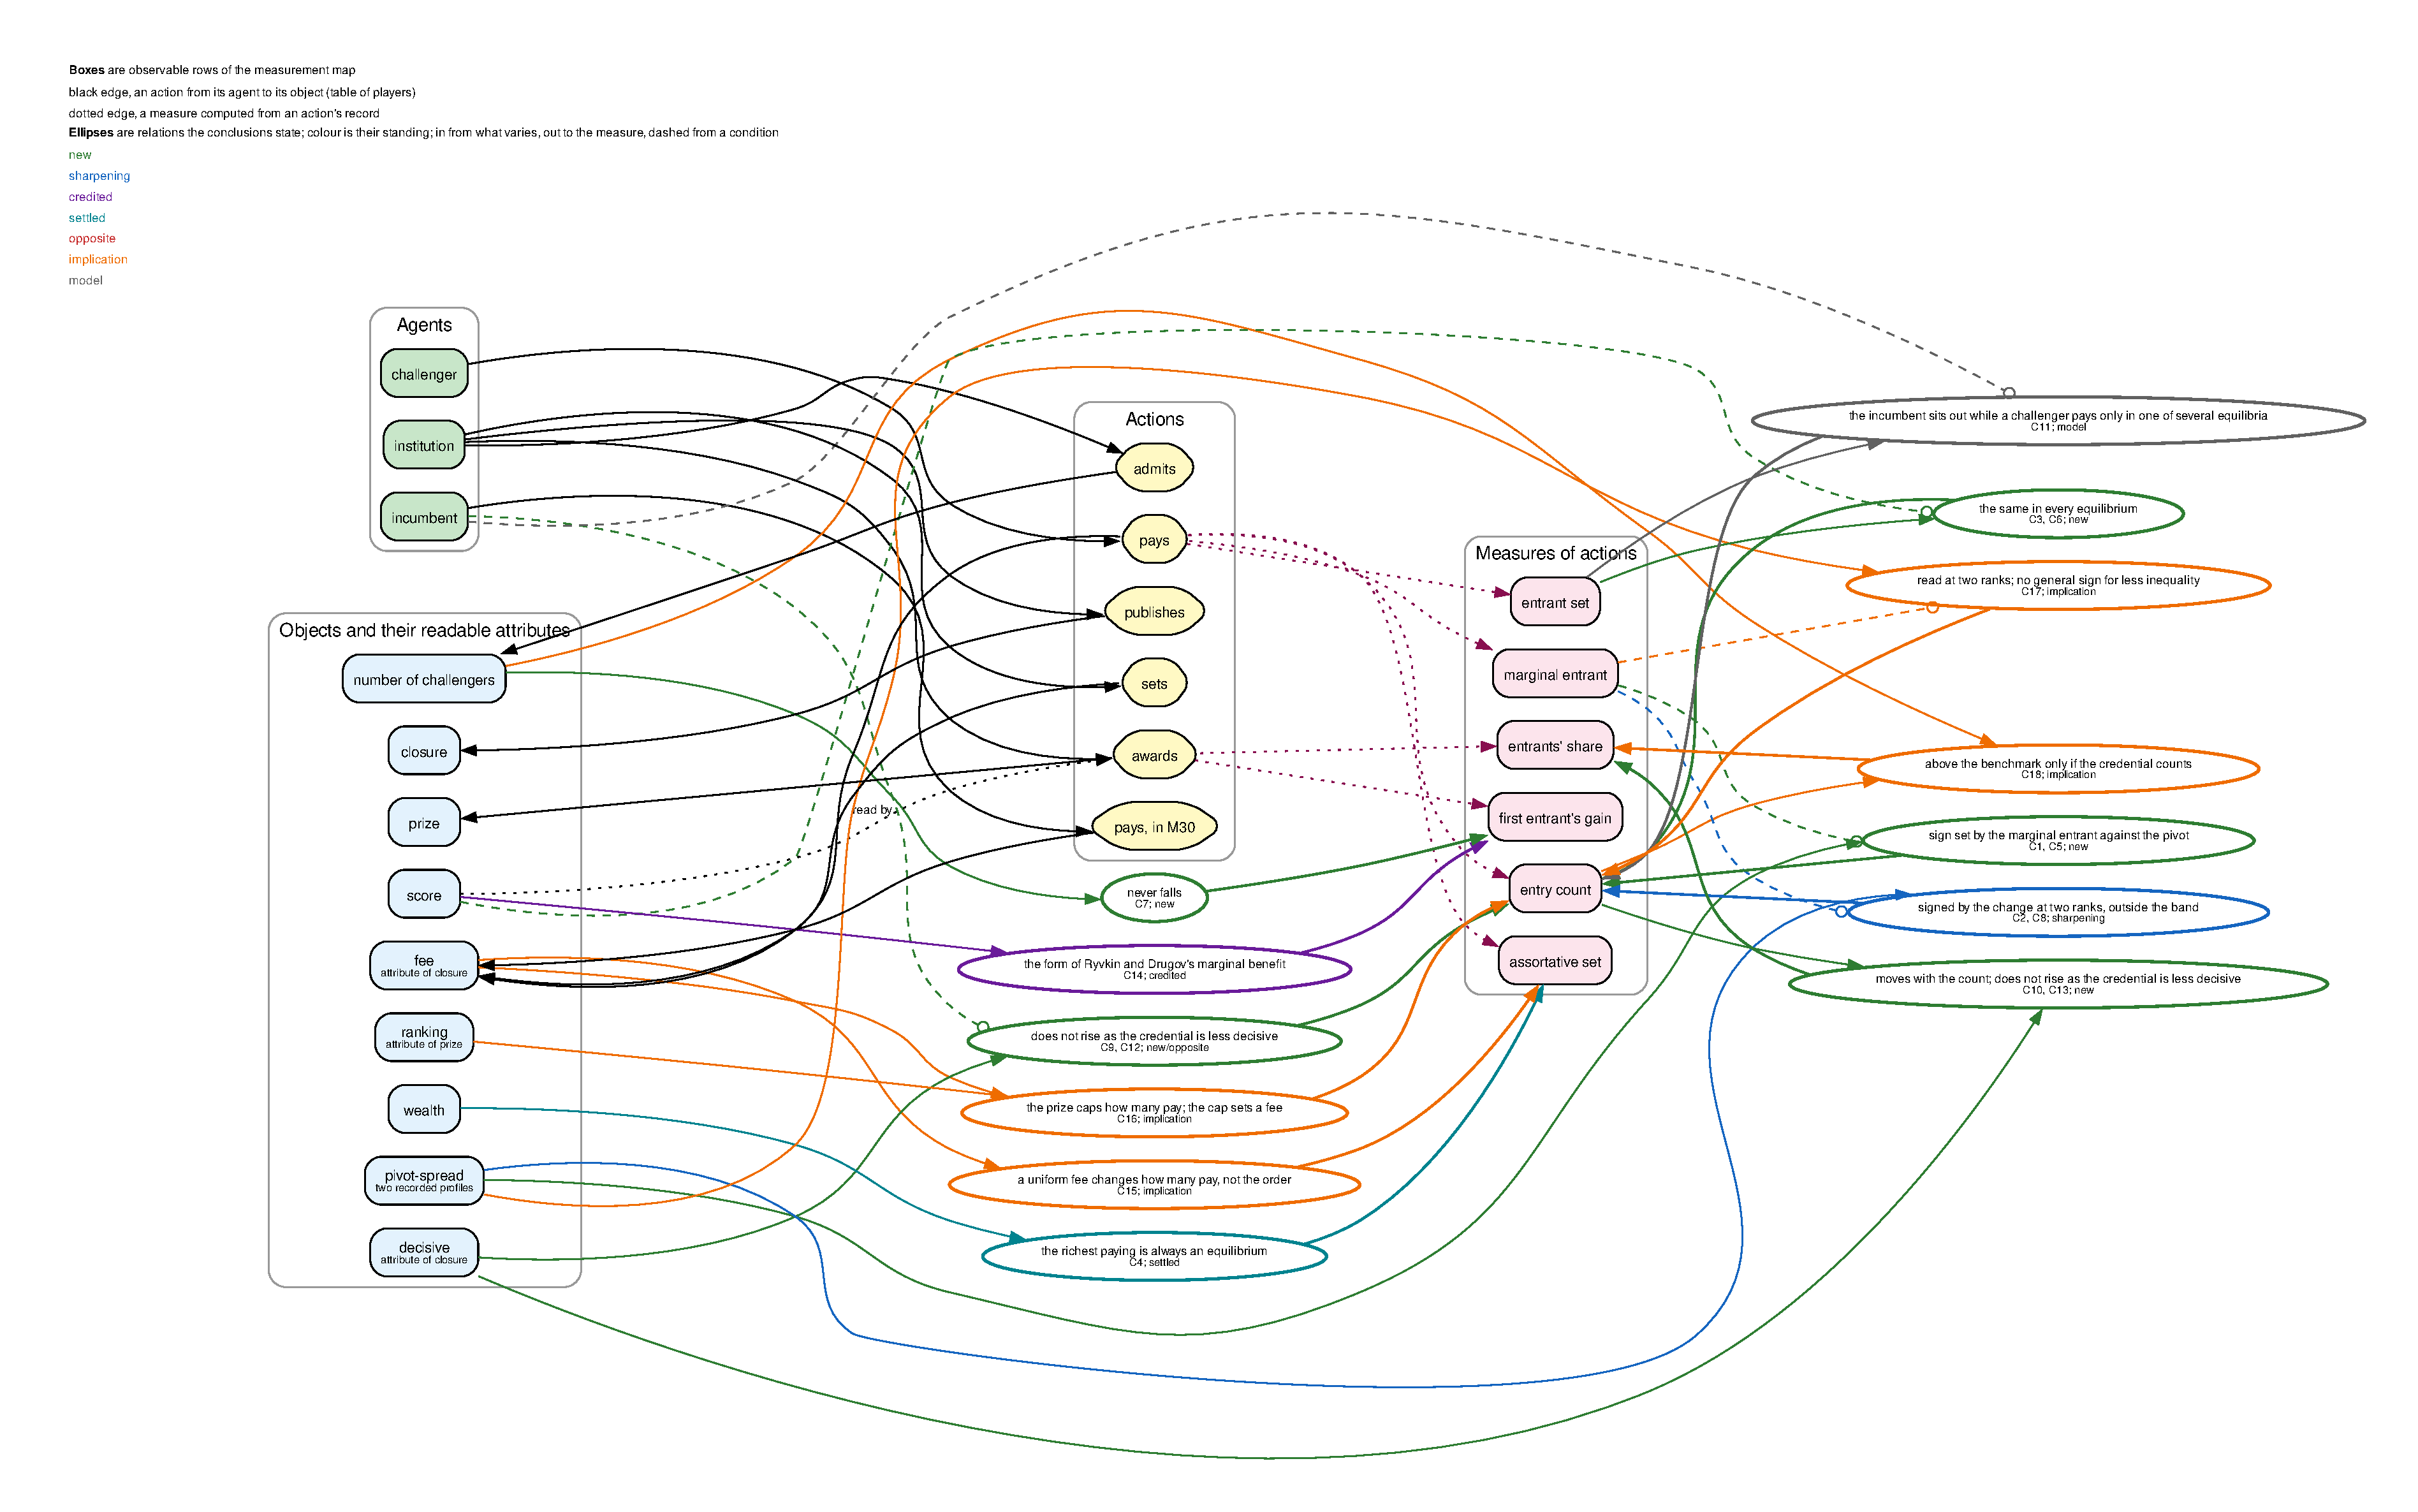
\includegraphics[angle=90,width=\textwidth,height=0.9\textheight,keepaspectratio]{figures/conclusions_ledger.pdf}
\caption{The conclusions as relations among observable entities. Boxes are rows
of the measurement map that an observer records or computes, in four columns,
the agents, the objects they act on with their readable attributes, the actions
and the measures of actions. A black edge runs from an agent through its action
to the object, as Table~\ref{tab:players} gives the option; a dotted edge leads
from an action to a measure computed from its record. Each ellipse is a relation
the conclusions state, labelled with what it says, the conclusions it represents
and their standing against the papers read; solid edges lead in from what varies
and out to the measure that responds, and dashed edges are conditions. The
figure is drawn by \texttt{checks/ledger\_literature.py} from its ledger
(Appendix~\ref{app:evidence}).}
\label{fig:ledger}
\end{figure}

\footnotesize
\begin{longtable}{@{}P{0.8cm}P{12.3cm}P{3.4cm}@{}}
\caption{Conclusions that rest on the model rows and on the papers read.}
\label{tab:concl}\\
\toprule
\textbf{ID} & \textbf{Statement} & \textbf{Rests on} \\
\midrule
\endfirsthead
\toprule
\textbf{ID} & \textbf{Statement} & \textbf{Rests on} \\
\midrule
\endhead
\bottomrule
\endfoot
\crow{C1}{For a fixed prize awarded by rank, a pivot-spread of wealth moves the
  number of entrants weakly, in a direction set by one comparison, the
  marginal entrant against the pivot of the spread. Given score laws that do
  not depend on who enters, the rule needs only that the fee's utility cost
  falls with wealth. In the privilege contest of Schroyen and Treich the effect
  of a spread on effort turns on $u'''$; on the entry margin the sign needs no
  condition on $u'''$. Their paper was read in its working-paper version (L12).}
  {M13, M23, M24, M26, L12}
\crow{C2}{The margin condition reads the wealth profile at two ranks only, the
  marginal entrant and the first outsider, and it holds for any change of
  profile, mean-preserving or not (M12). Where the marginal entrant becomes
  poorer and the first outsider richer, the signs of the change settle nothing,
  even for mean-preserving spreads, and the mean cannot stand in for the pivot
  (M13, M14). Costrell and Loury, in their two-job model, sign a spread by one
  marginal quantile fixed by technology (L9); here the margin is the count
  itself, which moves with the profile.}
  {M12, M13, M14, L9}
\crow{C3}{Every pure-strategy equilibrium has the same number of entrants
  because the gain depends on that number alone and does not rise with it (M4,
  M26). When the gain depends on who enters, the count need not be pinned: for
  some laws in which the bought component falls (M27) or rises (M29) with
  wealth it is not,
  and our witness in the entry stage of Fullerton and McAfee, where profits
  depend on rivals' costs, has two counts (L5). In the priority queue of
  Hassin and Haviv buying follows the crowd, the opposite monotonicity, and
  several equilibria can coexist (L31).}
  {M4, M6, M26, M27, M29, L5, L31}
\crow{C4}{Under complete information every pure-strategy equilibrium has $k^*$
  entrants (M6), as in pure strategies with identical entrants (L2, L3). With
  heterogeneous costs the $k^*$ richest entering is always an equilibrium
  (M8), so who enters is settled without the devices that models with
  identical entrants use for that purpose: mixed entry (L2), private random
  delays (L3) and sequential arrival (L7). Who enters is pinned when the
  condition of M7 holds, and need not be otherwise.}
  {M5, M6, M7, M8, L2, L3, L4, L7}
\crow{C5}{The sign rule of C1 is new among the papers read. None of the entry
  papers read signs the effect of a spread of wealth, or of a spread of entry
  costs, on the number of entrants at a fixed number of potential entrants. In
  \citet{CorcoranKarels1985}, whose players are identical, the count is set by
  the lottery's exponent, the commitment assumed or a minimum bet (L29). The
  privilege contest of C1 signs effort, not entry (L12). Fernández and Galí,
  a rank-order allocation in which wealth matters, fix the wealth distribution
  and sign no spread (L30).}
  {M13, L2, L3, L4, L5, L6, L7, L12, L23, L24, L29, L30}
\crow{C6}{Count invariance across pure-strategy equilibria with heterogeneous
  entry costs, for finitely many challengers, is new among the papers read. The
  entry papers read have identical entrants (Levin and Smith, Morgan, Orzen and
  Sefton, Fu, Jiao and Lu, Fu and Lu, Corcoran, Corcoran and Karels), a random
  count under private costs (Moreno and Wooders), or, in our witness for the
  entry stage of Fullerton and McAfee, a count that differs across equilibria.
  Mathews and Namoro fix the number of strategic entrants at two. In the
  continuum model of Fryer and Loury, with a binary investment and
  heterogeneous costs, the investment rate is unique and the investors are the
  agents below a cost threshold (L25), the continuum counterpart; with finitely
  many contestants the count is pinned (M6) while the identities need not be
  (the example in Appendix~\ref{app:primitives}, Information). In the continuum
  model of Coate and Loury the investment rate need not be unique, because the
  employer's standard responds to the rate it expects (L28); with the rule
  fixed, as here, that channel is absent. Under hit-and-run entry Corcoran and
  Karels find several stable counts, because incumbents choose among
  pre-emptive bets, not because entrants differ (L29). In Hassin and Haviv,
  identical customers buy priority at a fixed toll and several thresholds can
  be equilibria, because buying follows the crowd (L31).}
  {M6, M7, L2, L3, L4, L5, L6, L7, L23, L24, L25, L28, L29, L31}
\crow{C7}{Beyond what C14 credits to Ryvkin and Drugov, two statements about the
  first entrant's gain are new among the papers read. With a uniform base component
  it never falls in the number of challengers, because the peak of the score
  gap sits at the top of the outsiders' support, where the kernel vanishes,
  which it cannot do in their tournament (M18). For a bought component of two
  values, a shift condition on the base component makes the score gap single-peaked
  (M19). The search of 13 October 2026 found one candidate for these
  statements, \citet{FuLu2009}, whose investment is continuous and made by
  every contestant, so it is not a precedent (L26); the binary-investment
  models it also found, Fryer and Loury (L25) and Coate and Loury (L28), are
  continua with no number of challengers.}
  {M18, M19, L8, L25, L26, L28}
\crow{C8}{Outside the band, two ranks suffice to sign the change in the count
  (M12, M14), a sharpening of \citet{CostrellLoury2004}. Read in their
  published version, they sign a spread by one marginal quantile fixed by
  technology, or by the shape of the weight on ability, and never by two ranks
  (L9).}
  {M12, M14, L9}
\crow{C9}{With the fee, the prize and the wealth profile fixed, the number of
  entrants does not rise as the rule weighs the base component more, for every
  atomless law of the base component and every law of a non-negative bought
  component, when the incumbent is scored as an entrant. For an incumbent protected from the
  rule, whose law does not move with the weight, the argument does not apply
  (Appendix~\ref{app:primitives}). In the two effort models read the sign is
  the opposite (L20, L22): effort rises with the accuracy of the ranking until
  entry earns no more than staying out, while a fixed fee does not rise
  (Appendix~\ref{app:primitives}, ``No effort margin'').}
  {M28, L20, L22}
\crow{C10}{The share of the prize taken by the entrants is set by the count,
  so it moves weakly with the prize, the fee and the wealth profile in the
  direction the count does (M11 to M13), and it does not rise as the rule
  weighs the base component more. That a group with higher investment costs holds fewer
  positions is Fryer and Loury's result under laissez-faire, for identity
  groups in a continuum (L25); in Coate and Loury such a group does less well
  when employers set the standard (L28). The outcome is the opportunity hoarding
  of \citet{Tilly1998}, a bounded group keeping access to a valuable resource,
  read from one page (L19), but here no one hoards, and the fee and the wealth
  profile produce it. \citet{LaurisonFriedman2016} find access to the
  traditional professions more closed than to management, which pays more. Read
  as shares, a larger prize alone does not lower the share, so the prize does
  not account for that pattern; a rule weighing the bought component more is
  one difference consistent with it (weakly, M31), though the weight is not
  measured.}
  {M11, M12, M13, M28, M31, L17, L19, L25, L28}
\crow{C11}{An incumbent scored as an entrant, with the lowest cost, sits out
  while a challenger enters only as one of several equilibria with the same
  count, when $g(k^*)<\kappa_0$ and $\kappa_{k^*}\le g(k^*-1)$, and never when
  identities are pinned.}
  {M6, M7, M30}
\crow{C12}{The sign of M28 on the entry margin, for a rule that weighs the base
  component more, is new among the papers read. The two noise-comparative entry models
  read have the opposite sign, more noise bringing more entrants, because
  effort rises as noise falls and competes away the rents of entry above
  staying out (L20; Drugov and Ryvkin's free-entry extension, L22). M28's sign
  is that of their intensive margin, effort falling as noise becomes more
  dispersed (L22), which we read as the same margin, since entry, which buys
  the bought component, is the investment. The contrast with the number of
  challengers, which has no universal sign (M18, M20, M22), is theirs across
  their two papers (L8, L22). The working paper of Fryer and Loury conjectures,
  without deriving it, that a blind rule rationing slots at random lowers
  investment in both groups, the direction of M28; the published version drops
  the conjecture (L25). In the pair-wise tournaments of Fryer and Loury (2005)
  a blind redistribution rule creates a pool of contestants who exert no effort
  and still compete, and the pool grows as the redistribution target becomes
  more aggressive, which the paper asserts and the record derives (L27): the
  same direction, for a redistribution target rather than a weight on the base component,
  and with a continuous effort rather than a fee. In \citet{CoateLoury1993} a
  noisy test reads a binary investment, and in their uniform example, at a
  fixed employer policy, their formulas imply that both investment rates fall
  as the test becomes less accurate, a derivation of ours that the paper does
  not state (L28): the direction of M28 again, for the accuracy of a test and a
  standard that employers set. In \citet{FernandezGali1999}, as the signal
  grows more sensitive to the agents' endowment relative to their spending,
  aggregate spending tends to zero
  (L30): the direction of M28 again, as a limit, for a continuous expenditure
  in a continuum. The sign that is new is C9's: a fixed prize
  awarded by rank, a fixed fee, the incumbent scored as an entrant, and
  every atomless law of the base component and every law of a non-negative
  bought component.}
  {M18, M20, M22, M28, L8, L20, L22, L25, L27, L28, L30}
\crow{C13}{The share of the prize taken by those who enter, as a function of
  how many enter, and its comparative statics are new among the entry papers
  read. In Mathews and Namoro, non-strategic contestants fill the places that
  the strategic ones leave and can win, but they make no choice, the number of
  strategic contestants is fixed at two, and no share is analysed (L23). In
  every other entry model read, those who do not enter cannot win, so the share
  is not defined there; here outsiders compete on the base component. In the
  minimum-bet case of Corcoran and Karels every entrant wins with probability
  $1/n$ and those who do not bet cannot win (L29). Outside the entry
  literature, Fryer and Loury have a binary investment in which those who do
  not invest still compete, and the group with higher costs holds fewer slots
  (L25). Their agents form a continuum and slots are priced, so they do not
  derive the entrants' share as a function of how many enter, nor its comparative
  statics. In \citet{CoateLoury1993} those who do not invest can reach the
  better job and the assignment rate is split between investors and
  non-investors, but the number of places moves with the standard and the
  investors' share is not analysed (L28). In Fernández and Galí who spends
  nothing gets the lowest school (L30). In Hassin and Haviv those who do not
  buy priority are still served, but there is no prize to share (L31). The
  nearest construct is the access of Liu, Garg and Borgs, a group's admission
  probability for a fixed number of places, which does not rise as the ranking
  becomes more decisive; the group is fixed by environment and effort is
  continuous, so no share of those who pay is defined (L32). Hu, Immorlica and
  Vaughan give the errors of a threshold by group, with no fixed number of
  positions (L33).}
  {M31, L2, L3, L4, L5, L6, L7, L20, L22, L23, L24, L25, L28, L29, L30, L31, L32, L33}
\crow{C14}{The first entrant's gain is $V\,\mathbb E[\varphi(M)]$, with $M$ the
  best rival's score (M1). This is the form of the marginal benefit of
  \citet{RyvkinDrugov2020}, the noise density at the best rival's shock, with
  the score gap $\varphi$ in place of the density. Their Karlin step, with
  the law of $M$ in place of $F^{k-1}$, gives M17, no interior minimum in the
  number of challengers when $\varphi$ is single-peaked. Their remark that
  with many players the comparative statics follow the upper tail is what M21
  makes precise for the gain, in the class of M19.}
  {M1, M17, M21, L8}
\crow{C15}{A fee equal for every challenger changes how many enter, not the
  order in which they enter. At every fee the order of entry is the order of
  wealth (M5, M23), and in the equilibrium in which the richest enter a lower
  fee adds entrants from the next-richest down (M8, M11). Fees that differ
  across challengers can reverse the order of costs (M33), so only a fee that
  varies with the challenger can bring a poorer challenger in ahead of a
  richer one.}
  {M5, M8, M11, M23, M33}
\crow{C16}{The prize caps how many pay, and the cap sets a fee. At any fee at
  which $(k+1)\kappa_k$ exceeds $V$, at most $k$ challengers enter (M10, M33),
  so an institution that wants at most $k$ entrants needs only the prize and
  the cost of the fee to the $(k+1)$-th richest.}
  {M10, M33}
\crow{C17}{Whether a compression of wealth raises participation is read at two
  ranks. A compression toward a pivot weakly raises the count when the marginal
  entrant stands at or below the pivot, and weakly lowers it when the first
  outsider stands at or above it (M12, M33); inside the band between them the
  direction is not determined (M14). That less inequality brings more
  participation has no general sign, since a spread that keeps the mean can
  lower the count (M13).}
  {M12, M13, M14, M33}
\crow{C18}{A large share of positions among the holders of the bought
  component is not by itself evidence that it counts. When it adds nothing to
  the score, the entrants, the incumbent included, take $\frac{k+1}{Q+1}$ of
  the prize, their share of the players (M31). With a non-negative bought
  component the share is never below that benchmark, and a share off it means
  the two score laws differ (M33), so only a share above the benchmark shows
  that the bought component counts. This bears on how the opportunity hoarding
  of \citet{Tilly1998} is read in data (L19).}
  {M31, M33, L19}
\end{longtable}

\normalsize

\appendix

\section{Proofs}
\label{app:proofs}

\paragraph{Notation.} Challenger $i$ scores $\sigma_i=\mu r_i+(1-\mu)s_ie_i$, with
the base component $r_i$ and the bought component $s_i\ge0$ drawn independently
of each other and of wealth, $\mu$ the weight on the base component, and the fee
$c>0$. $F$ and $G$ are the score CDFs
of an entrant and of an outsider, and $C$ is the incumbent's, each without atoms.
With $m$ other entrants among the $Q$ challengers,
\[
  H_m=C\,F^{m}G^{Q-1-m},\qquad K_m=C\,F^{m}G^{Q-2-m},\qquad \varphi=G-F,
\]
\[
  \Delta(m)=V\Big(\int H_m\,dF-\int H_m\,dG\Big),\qquad \kappa(w)=u(w)-u(w-c).
\]
$H_m$ is the CDF of the best score facing a challenger, $M_m$ a random variable
with that CDF, and $K_m$ the same CDF with one more challenger set aside, so that
$H_{m+1}=K_mF$ and $H_m=K_mG$.
Challengers are indexed $0,\dots,Q-1$ in increasing order of cost,
$\kappa_0\le\dots\le\kappa_{Q-1}$, which is decreasing order of wealth. Index $j$
enters when $\kappa_j\le\Delta(j)$, and $k^*$ satisfies $\kappa_j\le\Delta(j)$ for
$j<k^*$ and $\Delta(k^*)<\kappa_{k^*}$ when $k^*<Q$. Past $Q-1$, $\Delta(m)$ means
$\Delta(Q-1)$; so extended, $\Delta$ is non-increasing on every count by M4, and
the results that use this cite M4. In the results on wealth
profiles, rank $j$ has wealth $w_j$ with $w_0\ge w_1\ge\cdots$, and enters when
$w_j>c$ and $\kappa(w_j)\le\Delta(j)$, so a challenger whose wealth is at or below
the fee does not enter. A prime marks the profile after a change and its count
$k'^*$. When the number of challengers varies, $\Delta_Q(0)$ is the first
entrant's gain among $Q$ challengers, with
\[
  D(Q)=\Delta_{Q+1}(0)-\Delta_Q(0),\qquad W_Q=C\,G^{Q-1}(1-G).
\]

\begin{mproof}{M1}{EntryContestP1P2.two_max_sum, EntryContestP1P2.p1_representation, EntryContestP1P2.Delta_eq_expectation}
For independent $X\sim A$ and $Y\sim B$ with $B$ atomless, $\Pr(X=Y)=0$, so
\[
  \int B\,dA+\int A\,dB=\Pr(Y\le X)+\Pr(X\le Y)=1 .
\]
With $(A,B)=(F,H_m)$ and $(A,B)=(G,H_m)$,
\[
  \int H_m\,dF=1-\int F\,dH_m,\qquad \int H_m\,dG=1-\int G\,dH_m ,
\]
so
\[
  \frac{\Delta(m)}{V}=\int (G-F)\,dH_m=\int\varphi\,dH_m=\mathbb E[\varphi(M_m)] .
\]
\end{mproof}

\begin{mproof}{M2}{EntryContestP1P2.p2_fosd, EntryContestP1P2.p2_strict_interval, EntryContestP1P2.Delta_nonneg_from_primitives}
Let $X=\mu r+(1-\mu)s$ and $Y=\mu r$. For $\mu\le1$ and $s\ge0$, $X-Y=(1-\mu)s\ge0$,
so $\{X\le x\}\subseteq\{Y\le x\}\cup\{s<0\}$ and
\[
  F(x)\le G(x)+\Pr(s<0)=G(x),\qquad \Delta(m)=V\!\int\varphi\,dH_m\ge0 .
\]
For $\mu<1$,
\[
  \{s>0\}\subseteq\{Y<X\}=\bigcup_{q\in\mathbb Q}\{Y\le q<X\},
\]
so $\Pr(s>0)>0$ gives $q\in\mathbb Q$ with $\Pr(Y\le q<X)>0$, and
\[
  G(q)\ge\Pr(X\le q)+\Pr(Y\le q<X)>F(q).
\]
$G-F$ is right-continuous, so $G-F>0$ on some $[q,u)$.
\end{mproof}

\begin{mproof}{M3}{EntryContestStep.three_max_sum_real, EntryContestStep.step_identity, EntryContestModel.Delta_step}
Write $K=K_m$, so $H_{m+1}=KF$ and $H_m=KG$. For independent atomless draws
$Z\sim K$, $X\sim A$, $Y\sim B$, exactly one is the largest,
\[
  \int AB\,dK+\int KB\,dA+\int KA\,dB=1 .
\]
With $(A,B)=(F,F)$, $(G,G)$ and $(F,G)$,
\[
  \int KF\,dF=\tfrac12\Big(1-\int F^2dK\Big),\quad
  \int KG\,dG=\tfrac12\Big(1-\int G^2dK\Big),\quad
  \int KG\,dF+\int KF\,dG=1-\int FG\,dK ,
\]
so
\[
  \frac{\Delta(m{+}1)-\Delta(m)}{V}
  =\int KF\,dF-\int KF\,dG-\int KG\,dF+\int KG\,dG
  =-\tfrac12\int (F-G)^2\,dK .
\]
\end{mproof}

\begin{mproof}{M4}{EntryContestModel.Delta_step_nonpos, EntryContestModel.DeltaUpTo_step, EntryContestEq.Delta_step_strict}
By M3 and $\varphi^2\ge0$,
\[
  \Delta(m{+}1)-\Delta(m)=-\tfrac V2\int\varphi^2\,dK_m\le0 \quad (V\ge0),
  \qquad <0 \quad \Big(V>0,\ \int\varphi^2\,dK_m>0\Big).
\]
Beyond $m=Q-1$ the gain is set to $\Delta(Q-1)$, so $\Delta(m{+}1)\le\Delta(m)$
for every $m$.
\end{mproof}

\begin{mproof}{M5}{EntryContest.single_crossing, EntryContestModel.p5_threshold_from_primitives}
For $i\le j$, by M4,
\[
  \kappa_i\le\kappa_j\le\Delta(j)\le\Delta(i).
\]
\end{mproof}

\begin{mproof}{M6}{EntryContestEq.count_invariance_fin, EntryContestMM.exists_mem_ge, EntryContestMM.exists_not_mem_le}
Let $S$ be an equilibrium and $k=|S|$. A $k$-set of indices has an element
$i\ge k-1$, since
$S\subseteq\{0,\dots,k-2\}$ gives $k\le k-1$, and omits some $j\le k$, since
$\{0,\dots,k\}\subseteq S$ gives $k+1\le k$. If $k>k^*$, then $k^*<Q$ and
\[
  \Delta(k^*)<\kappa_{k^*}\le\kappa_{k-1}\le\kappa_i\le\Delta(k-1)\le\Delta(k^*).
\]
If $k<k^*$, then $j<Q$ and
\[
  \Delta(k)<\kappa_j\le\kappa_k\le\Delta(k).
\]
Both are contradictions, so $k=k^*$.
\end{mproof}

\begin{mproof}{M7}{EntryContest.members_below_kstar, EntryContestEq.assortative_unique, EntryContestEq.assortative_only, EntryContestEq.assortative_only_model}
A member $i$ of an equilibrium has $\kappa_i\le\Delta(k^*-1)$ by M6. If $i\ge k^*$,
\[
  \kappa_i\ge\kappa_{k^*}>\Delta(k^*-1),
\]
so $i<k^*$. Then $S\subseteq\{0,\dots,k^*-1\}$ and $|S|=k^*$ give
$S=\{0,\dots,k^*-1\}$, an equilibrium by M8. With $\Delta$ the model's gain,
non-increasing by M4, nothing further is assumed.
\end{mproof}

\begin{mproof}{M8}{EntryContestEq.assortative_is_equilibrium, EntryContestEq.assortative_min_cost, EntryContestEq.prize_term_anonymous, EntryContestEq.payoff_gap_anonymous}
(i) For $i<k^*$ and for $k^*\le j<Q$,
\[
  \kappa_i\le\kappa_{k^*-1}\le\Delta(k^*-1),\qquad \Delta(k^*)<\kappa_{k^*}\le\kappa_j .
\]
(ii) Induct on $S$, adding its largest element $a$ last. With $T=S\setminus\{a\}$
and $T\subseteq\{0,\dots,a-1\}$, $|T|\le a$, so
\[
  \sum_{i<|T|+1}\kappa_i=\sum_{i<|T|}\kappa_i+\kappa_{|T|}
  \le\sum_{i\in T}\kappa_i+\kappa_a=\sum_{i\in S}\kappa_i .
\]
(iii) With identical laws, the win probability of $i$ is
$P^{\mathrm{in}}(|S|)=\int CF^{|S|-1}G^{Q-|S|}\,dF$ for $i\in S$ and
$P^{\mathrm{out}}(|S|)=\int CF^{|S|}G^{Q-1-|S|}\,dG$ for $i\notin S$, so with
$EU_i(S)=u(w_i)-\kappa_i\mathbf 1\{i\in S\}+V P_i(S)$,
\[
  \sum_iEU_i(S)=\sum_iu(w_i)-\sum_{i\in S}\kappa_i
  +V\big(|S|P^{\mathrm{in}}(|S|)+(Q-|S|)P^{\mathrm{out}}(|S|)\big),
\]
and the last term is the same for any two entrant sets of one size.
\end{mproof}

\begin{mproof}{M9}{EntryContestP6P7.integral_iid, EntryContestP6P7.integral_cdf_pow, EntryContestP6P7.p6_evaluation, EntryContestP6P7.p6_at_zero, EntryContestP6P7.tendsto_cdf_investorLaw, EntryContestP6P7.tendsto_cdf_nonInvestorLaw, EntryContestP6P7.p6_limit}
For $X_0,\dots,X_k$ independent with atomless CDF $F$,
\[
  \int F^k\,dF=\Pr\Big(X_0=\max_{i\le k}X_i\Big)=\frac1{k+1}.
\]
At $\mu=0$ the entrant scores $s$ and the outsider $0$, so
$G=\mathbf 1_{[0,\infty)}$ and $F(0)=\Pr(s\le0)=0$. With $C=F$,
\[
  \int H_m\,dF=\int F^{m+1}\,dF=\frac1{m+2},\qquad \int H_m\,dG=H_m(0)=0 .
\]
For $\mu\to0$ let $X_\mu=\mu r+(1-\mu)s$ and $Y_\mu=\mu r$. For $s>0$,
\[
  F_\mu(X_\mu)\to F_0(s),\qquad G_\mu(X_\mu)\to1,\qquad F_\mu(Y_\mu)\to F_0(0)=0,
\]
with every integrand in $[0,1]$, so by dominated convergence
\[
  \int H_m\,dF_\mu\to\int F_0^{m+1}\,dF_0=\frac1{m+2},\qquad
  0\le\int H_m\,dG_\mu\le\mathbb E\big[F_\mu(Y_\mu)\big]\to0 .
\]
\end{mproof}

\begin{mproof}{M10}{EntryContestP6P7.integral_cdf_pow, EntryContestP6P7.p7_Delta_le, EntryContestP6P7.p7_cap, EntryContestP6P7.p7_count}
From $C\le1$, $G\le1$ and $\int H_m\,dG\ge0$,
\[
  \Delta(m)\le V\int H_m\,dF\le V\int F^m\,dF=\frac V{m+1}.
\]
For $\kappa\le\Delta(m)$,
\[
  (m+1)\,\kappa\le(m+1)\,\Delta(m)\le V,\qquad m+1\le\frac V\kappa\quad(\kappa>0),
\]
and a member $i$ of an equilibrium $S$ has $\kappa_i\le\Delta(|S|-1)$, so
$|S|\,\kappa_i\le V$.
\end{mproof}

\begin{mproof}{M11}{EntryContestSpread.count_ge_of_enters, EntryContestSpread.count_mono_gain, EntryContestSpread.count_mono_prize, EntryContestEq.Delta_mono_prize, EntryContestMM.Delta_scale, EntryContestSpread.count_antitone_fee}
Rank $j$ enters when $c<w_j$ and $\kappa(w_j)\le\Delta(j)$, and $k^*$ is the length of
the prefix of entrants. If every rank $j<k'$ enters under $(\kappa,\Delta)$ then
$k'\le k^*$. Write $\Delta_V$ for the gain at prize $V$. By M1 and M2,
\[
  \Delta_V(j)=V\,\Delta_1(j),\quad \Delta_1(j)\ge0\quad(\mu\le1,\ s\ge0),\qquad
  V\le V'\ \Rightarrow\ \Delta_V(j)\le\Delta_{V'}(j),
\]
so an entrant at $V$ enters at $V'$. For $c\le c'$ and $c'<w_j$,
\[
  c<w_j,\qquad 0<w_j-c'\le w_j-c\ \Rightarrow\ u(w_j)-u(w_j-c)\le u(w_j)-u(w_j-c'),
\]
so an entrant at $c'$ enters at $c$.
\end{mproof}

\begin{mproof}{M12}{EntryContestSpread.enters_down, EntryContestSpread.count_ge_of_enters, EntryContestSpread.count_le_of_fails, EntryContestSpread.margin_rise, EntryContestSpread.margin_fall}
(i) The marginal entrant has $c<w_{k^*-1}\le w'_{k^*-1}$, so
\[
  \kappa(w'_{k^*-1})\le\kappa(w_{k^*-1})\le\Delta(k^*-1),
\]
and for $i\le k^*-1$, with $w'_i\ge w'_{k^*-1}>c$,
\[
  \kappa(w'_i)\le\kappa(w'_{k^*-1})\le\Delta(k^*-1)\le\Delta(i).
\]
Every $i<k^*$ enters after the change, so $k^*\le k'^*$.
(ii) For $k^*<Q$, rank $k^*$ fails before the change. If $w'_{k^*}>c$, then
$c<w'_{k^*}\le w_{k^*}$ and
\[
  \kappa(w'_{k^*})\ge\kappa(w_{k^*})>\Delta(k^*),
\]
so rank $k^*$ fails after the change and $k'^*\le k^*$.
\end{mproof}

\begin{mproof}{M13}{EntryContestSpread.pivot_rise, EntryContestSpread.pivot_fall, EntryContestSpread.spread_isPivot, EntryContestMM.mm2a, EntryContestSpread.mps_lowers_count, EntryContestSpread.mps_lowers_witness_counts, EntryContestSpread.mps_lowers_count_positive}
$T$ is non-decreasing, so $w'_j=T(w_j)$ is sorted, and
\[
  x_0\le w_{k^*-1}\ \Rightarrow\ w_{k^*-1}\le T(w_{k^*-1}),\qquad
  w_{k^*}\le w_{k^*-1}\le x_0\ \Rightarrow\ T(w_{k^*})\le w_{k^*},
\]
so M12 applies. For $T(w)=x_0+\lambda(w-x_0)$ with $\lambda\ge1$,
\[
  T(w)-w=(\lambda-1)(w-x_0),\qquad
  \frac1Q\sum_jT(w_j)=\bar w+\lambda\Big(\frac1Q\sum_jw_j-\bar w\Big)=\bar w
  \quad (x_0=\bar w).
\]
With $c=1$, $\kappa(w)=\frac1{w-1}-\frac1w$ and $\Delta(m)=\frac1{m+2}$,
\[
  w=\big(\tfrac{29}{10},\tfrac{14}5,2\big),\quad
  w'=\big(\tfrac{18}5,\tfrac{11}5,\tfrac{19}{10}\big),\quad
  \textstyle\sum_jw_j=\sum_jw'_j,\quad w'_2\le w_2,\quad w'_2+w'_1\le w_2+w_1,
\]
\[
  \kappa(w)=\big(\tfrac{100}{551},\tfrac{25}{126},\tfrac12\big),\quad
  \kappa(w')=\big(\tfrac{25}{234},\tfrac{25}{66},\tfrac{100}{171}\big),\quad
  \tfrac13\textstyle\sum_jw_j=\tfrac{77}{30}<w_1,
\]
so the counts are $2$ and $1$. They hold for any $\Delta$ with
\[
  \tfrac{100}{551}\le\Delta(0),\quad \tfrac{25}{126}\le\Delta(1)<\tfrac{25}{66},\quad
  \Delta(2)<\tfrac12,
\]
strict at $\Delta(m)=\frac1{m+2}$, so by M9 they hold for every small $\mu>0$ with
$r$ and $s$ uniform.
\end{mproof}

\begin{mproof}{M14}{EntryContestSpread.branch_of_not_band, EntryContestSpread.not_band_of_single_crossing, EntryContestSpread.pivot_single_crossing, EntryContestSpread.mps_band_signs, EntryContestSpread.mps_witness_counts, EntryContestSpread.mps_band_both_directions, EntryContestSpread.mps_band_both_directions_positive}
Outside the band $d_{k^*-1}\ge0$ or $d_{k^*}\le0$, and M12 signs the change. If
\[
  i\le j,\ d_j>0\ \Rightarrow\ d_i\ge0,
\]
then $d_{k^*}>0$ gives $d_{k^*-1}\ge0$. A pivot-spread has this property, since
$d_j>0$ gives $w_j>x_0$ and then $w_i\ge w_j>x_0$. With $\kappa$ and $\Delta$ as
in M13, the profiles
\[
  w=\big(4,\tfrac{14}{5},\tfrac{11}{5},2\big),\quad
  w'=\big(\tfrac{41}{10},\tfrac{27}{10},\tfrac{13}{5},\tfrac85\big),\quad
  w''=\big(\tfrac{23}5,\tfrac94,\tfrac94,\tfrac{19}{10}\big)
\]
all sum to $11$, with partial sums from the poorest up
\[
  \big(2,\tfrac{21}5,7\big),\quad
  \big(\tfrac85,\tfrac{21}5,\tfrac{69}{10}\big),\quad
  \big(\tfrac{19}{10},\tfrac{83}{20},\tfrac{32}5\big),
\]
and
\[
  \kappa(w)=\big(\tfrac1{12},\tfrac{25}{126},\tfrac{25}{66},\tfrac12\big),\quad
  \kappa(w')=\big(\tfrac{100}{1271},\tfrac{100}{459},\tfrac{25}{104},\tfrac{25}{24}\big),\quad
  \kappa(w'')=\big(\tfrac{25}{414},\tfrac{16}{45},\tfrac{16}{45},\tfrac{100}{171}\big)
\]
against $\Delta=\big(\tfrac12,\tfrac13,\tfrac14,\tfrac15\big)$. The counts are
$2$, $3$ and $1$, and $d'$ and $d''$ both have signs $(+,-,+,-)$. Every
inequality is strict, so by M9 the counts hold for every small $\mu>0$.
\end{mproof}

\begin{mproof}{M15}{EntryContestKappa.exit_below_pivot, EntryContestKappa.enters_downward, EntryContestKappa.p9_strict, EntryContestKappa.p9_monotone, EntryContestKappa.p9_strict_model}
Let $j$ be an entrant at $\lambda=1$ with $w_j<x_0$. Since $\kappa(v)\to\infty$ as
$v\downarrow c$, some $u>c$ has $\kappa>\Delta(j)$ on $(c,u)$, and
\[
  \lambda>\bar\lambda=\max\Big(1,\frac{x_0-u}{x_0-w_j}\Big)
  \ \Rightarrow\ x_0+\lambda(w_j-x_0)<u ,
\]
so rank $j$ fails at $\lambda$. By the prefix property no rank from $j$ on
enters, and
\[
  k^*(\lambda)\le j<j+1\le k^*(1).
\]
For $1\le\lambda_1\le\lambda_2$, ranks with $w_i\ge x_0$ have $i<j$ and enter at
$\lambda_1$, while ranks with $w_i<x_0$ have
$x_0+\lambda_2(w_i-x_0)\le x_0+\lambda_1(w_i-x_0)$, so every entrant at
$\lambda_2$ enters at $\lambda_1$.
\end{mproof}

\begin{mproof}{M16}{EntryContestPMU.weight_eq, EntryContestPMU.pmu_identity, EntryContestPMU.pmu_sign_iff, EntryContestPMU.kernel_rises, EntryContestPMU.kernel_falls, EntryContestPMU.kernel_max}
With no other entrant, $H_0=CG^{Q-1}$ among $Q$ challengers and $CG^{Q}$ among
$Q+1$, and $CG^{Q-1}-CG^{Q}=W_Q$, so
\[
  \frac{D(Q)}V=\int\big(CG^{Q}-CG^{Q-1}\big)\,dF-\int\big(CG^{Q}-CG^{Q-1}\big)\,dG
  =-\Big(\int W_Q\,dF-\int W_Q\,dG\Big).
\]
For the kernel,
\[
  \frac{d}{dg}\,g^n(1-g)=g^{n-1}\big(n-(n+1)g\big)\quad(n\ge1),\qquad
  \frac{d}{dg}\,(1-g)=-1\quad(n=0).
\]
\end{mproof}

\begin{mproof}{M17}{EntryContestPMU.weight_shift, EntryContestPMU.pmu_single_crossing, EntryContestPMU.pmu_step_nonpos_persists, EntryContestPMU.quasiconcave_of_steps, EntryContestPMU.pmu_quasiconcave}
Let $k=Q_2-Q_1$, $\rho=G(x_0)^k$ and $\nu=dF-dG$. By M16 and $W_{Q_2}=G^kW_{Q_1}$,
\[
  D(Q_2)-\rho\,D(Q_1)=-V\int\big(G^k-\rho\big)\,W_{Q_1}\,d\nu .
\]
$G$ is non-decreasing and $W_{Q_1}\ge0$, so
\[
  \big(G^k-\rho\big)W_{Q_1}\le0,\ \nu\le0\ \text{on }(-\infty,x_0],\qquad
  \big(G^k-\rho\big)W_{Q_1}\ge0,\ \nu\ge0\ \text{on }(x_0,\infty),
\]
and $D(Q_2)\le\rho\,D(Q_1)$. Then $D(i)\le0$ gives $D(j)\le0$ for $j\ge i$. If
$D(i)\le0$ for some $Q_1\le i<Q_2$, then $\Delta_{Q_3}(0)\le\Delta_{Q_2}(0)$, and
otherwise $\Delta_{Q_1}(0)\le\Delta_{Q_2}(0)$.
\end{mproof}

\begin{mproof}{M18}{EntryContestPMU.uniform_left, EntryContestPMU.uniform_right, EntryContestPMU.pmu_quasiconcave_uniform, EntryContestRefute.pmu_step_nonneg_uniform, EntryContestRefute.Delta_mono_uniform}
$G$ is the law of $\mu r$, so $G=1$ on $[\mu,\infty)$, $dG=0$ on $(\mu,\infty)$
and $W_Q=0$ there. For $B\subseteq(-\infty,\mu]$ and $y\ge0$, with
$\tau=(1-\mu)y/\mu$ and $\lambda$ Lebesgue measure,
\[
  \Pr\big(\mu r+(1-\mu)y\in B\big)=\lambda\Big([\tau,1]\cap\tfrac B\mu\Big)
  \le\lambda\Big([0,1]\cap\tfrac B\mu\Big)=\Pr(\mu r\in B),
\]
so $dF\le dG$ on $(-\infty,\mu]$ and M17 applies at $x_0=\mu$. By M16,
\[
  \frac{D(Q)}V=\int_{(-\infty,\mu]}W_Q\,d(G-F)\ge0 .
\]
\end{mproof}

\begin{mproof}{M19}{EntryContestShift.left_of_lift, EntryContestShift.right_of_lift, EntryContestShift.quasiconcave_of_shiftMono, EntryContestShift.shiftMono_of_density, EntryContestShift.lawA_shiftMono, EntryContestShift.witness_quasiconcave}
Let $t=1-\mu$ and $G_t$ be the law of $\mu r+t$, so $F=pG+(1-p)G_t$. From
$\Pr(r\le0)=0$, $G_t$ has no mass on $(-\infty,t]$, where $dF=p\,dG\le dG$. For
$B\subseteq(t,\infty)$, with $c=t/\mu$ and $B/\mu\subseteq(c,\infty)$,
\[
  G(B)=\Pr\big(r\in\tfrac B\mu\big)\le\Pr\big(r\in\tfrac B\mu-c\big)=G_t(B),
\]
so $dF\ge dG$ on $(t,\infty)$ and M17 applies at $x_0=t$. For a density $g$
non-increasing on $(0,\infty)$ and $B\subseteq(c,\infty)$,
\[
  \int_B g(x)\,dx\le\int_B g(x-c)\,dx=\int_{B-c}g(x)\,dx ,
\]
and the smaller of two uniform draws has $\Pr(r\le x)=1-(1-x)^2$ and density
$2(1-x)$ on $[0,1]$.
\end{mproof}

\begin{mproof}{M20}{EntryContestFall.stepQ_one, EntryContestFall.stepQ_two, EntryContestFall.rise_then_fall, EntryContestFall.fall_from_one}
Here $G(x)=1-\big(1-\tfrac{4x}3\big)^2$ on $[0,\frac34]$,
$F(x)=pG(x)+(1-p)G(x-\frac14)$, $W_1=F(1-G)$ and $W_2=FG(1-G)$. By M16, integrating
the piecewise polynomials on $[0,\frac14]$, $[\frac14,\frac34]$ and $[\frac34,1]$,
\[
  \frac{D(1)}V=-\frac{11p^2}{162}+\frac{1901p}{21870}-\frac{208}{10935},\qquad
  \frac{D(2)}V=-\frac{4933p^2}{393660}+\frac{77219p}{2755620}-\frac{10672}{688905},
\]
so
\[
  p=\tfrac12:\ \frac{D(1)}V=\frac{653}{87480},\ \ \frac{D(2)}V=-\frac{10169}{2204496},
  \qquad p=\tfrac14:\ \frac{D(1)}V=-\frac{179}{116640}.
\]
\end{mproof}

\begin{mproof}{M21}{EntryContestMustFall.must_fall_general, EntryContestMustFall.shift_dominates, EntryContestMustFall.stepQ_bern, EntryContestMustFall.must_fall, EntryContestMustFall.witness_must_fall, EntryContestMustFall.unif_shiftMono, EntryContestMustFall.uniform_never_gains}
With $F=pG+(1-p)G_t$ and $W_Q=G^{Q-1}W_1$, M16 gives
\[
  D(Q)=-V(1-p)\Big(\int W_Q\,dG_t-\int W_Q\,dG\Big).
\]
$G_t$ has no mass on $(-\infty,t]$, $dG_t\ge dG$ on $(t,\infty)$ by M19, and
$W_1\ge\eta=C(a)\big(1-G(b)\big)>0$ on $(a,b]$. Splitting at $t$ and $a$,
\[
  \int W_Q\,dG_t-\int W_Q\,dG\ \ge\ G(a)^{Q-1}A-G(t)^{Q-1}B,
\]
\[
  A=\int_{(a,\infty)}W_1\,d(G_t-G)\ge\eta\,(G_t-G)\big((a,b]\big)>0,\qquad
  B=\int_{(-\infty,t]}W_1\,dG\ge0 .
\]
With $r_0=G(t)/G(a)<1$ and $r_0^{Q_0-1}(B+1)<A$, the bound is positive for
$Q\ge Q_0$. For M20's base law, $t=\frac14$ and
\[
  G\big((\tfrac12,\tfrac58]\big)=\tfrac{35}{36}-\tfrac89=\tfrac1{12}
  <\tfrac7{36}=\tfrac34-\tfrac59=G_t\big((\tfrac12,\tfrac58]\big).
\]
A uniform base component is shift-monotone, and M18 gives $D(Q)\ge0$, so it never
meets the condition.
\end{mproof}

\begin{mproof}{M22}{EntryContestPMUWitness.pairA_fosd, EntryContestPMUWitness.pairB_fosd, EntryContestPMUWitness.pairA_step_one, EntryContestPMUWitness.pairA_step_two, EntryContestPMUWitness.pairB_step, EntryContestPMUWitness.fosd_does_not_sign}
Pair one, with $y=1-x$, $W_1=x(1-x)^2$, $W_2=x\big(1-(1-x)^2\big)(1-x)^2$ and
$dG=2(1-x)\,dx$, gives
\[
  \int W_1\,dF=\tfrac1{12},\quad \int W_1\,dG=\tfrac1{10},\quad
  \int W_2\,dF=\int_0^1(y^2-y^3-y^4+y^5)\,dy=\tfrac1{20},\quad
  \int W_2\,dG=\tfrac{11}{210},
\]
\[
  \frac{D(1)}V=\tfrac1{10}-\tfrac1{12}=\tfrac1{60},\qquad
  \frac{D(2)}V=\tfrac{11}{210}-\tfrac1{20}=\tfrac1{420}.
\]
Pair two, with $W_Q=x^{Q+1}-x^{Q+2}$ and $dF=2x\,dx$, gives
\[
  \int W_Q\,dF=\frac2{(Q+3)(Q+4)},\qquad \int W_Q\,dG=\frac1{(Q+2)(Q+3)},\qquad
  \frac{D(Q)}V=-\frac{2(Q+2)-(Q+4)}{(Q+2)(Q+3)(Q+4)} .
\]
\end{mproof}

\begin{mproof}{M23}{EntryContestKappa.burden_strictAnti_of_strictConcave, EntryContestBM.burden_strictAnti_of_deriv, EntryContestBM.not_burden_of_convex_stretch, EntryContestKappa.log_burden_strictAnti, EntryContestKappa.crra_strictConcave, EntryContestKappa.crra_burden_strictAnti}
For $u$ strictly concave and $c<a<b$, secant slopes fall as either end moves
right, and $a-c<a<b$, $a-c<b-c<b$ give
\[
  \frac{u(a)-u(a-c)}{c}>\frac{u(b)-u(a-c)}{b-a+c}>\frac{u(b)-u(b-c)}{c},
\]
so $\kappa(a)>\kappa(b)$. With $u$ differentiable,
\[
  \kappa'(w)=u'(w)-u'(w-c)<0\quad(w>c).
\]
If $u$ is convex on $[a,b]$ with $b-a>c$, then $a<b-c$ and
\[
  \kappa(a+c)=u(a+c)-u(a)\le u(b)-u(b-c)=\kappa(b).
\]
Log and $x^{1-\gamma}/(1-\gamma)$ have $u''<0$ on $(0,\infty)$.
\end{mproof}

\begin{mproof}{M24}{EntryContestBM.rampU_burden, EntryContestBM.rampU_kappa_diverges, EntryContestBM.rampU_strictConvex, EntryContestBM.rampU_not_concave, EntryContestBM.admissibleParams_open, EntryContestBM.rampU_admissible, EntryContestBM.admissible_width, EntryContestBM.bm_strictly_weaker}
Let $\rho$ rise linearly from $0$ at $x_0$ to $1$ at $x_0+\sigma$, and
\[
  u(x)=\log x+x+\eta\int_0^x\rho(t)\,dt,\qquad u'(x)=\tfrac1x+1+\eta\rho(x)>0 .
\]
On $[x_0,x_0+\sigma]$, $u''=-x^{-2}+\eta/\sigma>0$ when $\sigma<\eta x_0^2$, so $u$
is strictly convex there and not concave. For $w>c$, $\rho(w)-\rho(w-c)\in[0,1]$
and vanishes unless $x_0<w<x_0+\sigma+c$, where
\[
  \tfrac1{w-c}-\tfrac1w=\tfrac c{w(w-c)}>\tfrac c{(x_0+\sigma+c)(x_0+\sigma)}>\eta ,
\]
so $u'(w)<u'(w-c)$ and M23 applies. $u(x)\to-\infty$ as $x\downarrow0$, so M25
gives the divergence. The conditions
\[
  x_0>0,\quad \sigma>0,\quad \sigma<\eta x_0^2,\quad \eta(x_0+\sigma+c)(x_0+\sigma)<c
\]
are strict inequalities in continuous functions, so they define an open set,
and for $\sigma<c$ an $\eta$ between $\sigma/x_0^2$ and
$c/\big((x_0+\sigma+c)(x_0+\sigma)\big)$ exists once $x_0$ is large, since
$\sigma(x_0+\sigma+c)(x_0+\sigma)/x_0^2\to\sigma<c$.
\end{mproof}

\begin{mproof}{M25}{EntryContestKappa.kappa_diverges_iff, EntryContestKappa.not_diverges_of_continuousWithinAt_zero, EntryContestKappa.log_kappa_diverges, EntryContestKappa.crra_kappa_diverges, EntryContestKappa.crra_kappa_not_diverges}
$u(w)\to u(c)$ as $w\downarrow c$, so
\[
  \kappa(w)=u(w)-u(w-c)\to\infty\iff u(w-c)\to-\infty\iff u(x)\to-\infty\ (x\downarrow0).
\]
$\log x\to-\infty$, and
\[
  \frac{x^{1-\gamma}}{1-\gamma}\to-\infty\quad(\gamma>1),\qquad
  \frac{x^{1-\gamma}}{1-\gamma}\to0\quad(\gamma<1).
\]
\end{mproof}

\begin{mproof}{M26}{EntryContestAnon.profile_mem, EntryContestAnon.profile_not_mem, EntryContestAnon.cdf_profile, EntryContestAnon.gain_anonymous}
Challenger $i$ wins with probability $\int C\prod_{j\ne i}L_j\,dL_i$, where $L_j$ is
$F$ for an entrant and $G$ for an outsider. With $|T|=m$ and $i\notin T$,
\[
  \frac{\mathrm{gain}_i(T)}V=\int CF^mG^{Q-1-m}\,dF-\int CF^mG^{Q-1-m}\,dG
  =\int H_m\,dF-\int H_m\,dG=\frac{\Delta(m)}V .
\]
\end{mproof}

\begin{mproof}{M27}{EntryContestAnon.winProb_zero_entrant, EntryContestAnon.winProb_zero_outsider, EntryContestAnon.gain_zero, EntryContestAnon.kappa3_values, EntryContestAnon.gains3, EntryContestAnon.anon_witness_zero, EntryContestAnon.gain_tendsto, EntryContestAnon.anon_witness_positive, EntryContestAnon.anon_witness_exists}
Let $r$ be uniform on $[0,1]$, entrant $j$'s $s_j$ the largest of $n_j$ uniform
draws, the incumbent's the largest of one, and $\mu=0$. An outsider scores $0$, and among the
$1+\sum_{j\in S}n_j$ draws each is equally likely to be the largest, so
\[
  \Pr(i\text{ wins})=\frac{n_i}{1+\sum_{j\in S}n_j},\qquad
  \mathrm{gain}_i(T)=\frac{V\,n_i}{1+n_i+\sum_{j\in T}n_j}.
\]
With $V=1$, $c=1$, $u(x)=-1/x$, $w=(\frac{11}4,\frac94,2)$ and $n=(1,2,3)$,
\[
  \kappa=\big(\tfrac{16}{77},\tfrac{16}{45},\tfrac12\big),\qquad
  \mathrm{gain}_2(\emptyset)=\tfrac34,\ \mathrm{gain}_0(\{2\})=\tfrac15,\
  \mathrm{gain}_1(\{2\})=\tfrac13,
\]
\[
  \mathrm{gain}_0(\{1\})=\tfrac14,\ \mathrm{gain}_1(\{0\})=\tfrac12,\
  \mathrm{gain}_2(\{0,1\})=\tfrac37,
\]
so $\{2\}$ and $\{0,1\}$ are equilibria. Every inequality is strict and each
gain is continuous in $\mu$ at $0$, so both remain equilibria for small $\mu>0$.
\end{mproof}

\begin{mproof}{M28}{EntryContestMu.Delta_normalise, EntryContestMu.cdf_payerLaw_antitone, EntryContestMu.first_integral, EntryContestMu.Delta_payer_mono, EntryContestMu.Delta_antitone_mu, EntryContestMu.kstar_antitone_mu}
For $\mu>0$ put $t=(1-\mu)/\mu$, $F_t$ the law of $r+ts$ and $G$ the law of
$r$. Dividing every score by $\mu$ changes no rank, so with $C=F$ and
$n=Q-1-m$,
\[
  \Delta(m;\mu)=V\Big(\int F_t^{\,m+1}G^{\,n}\,dF_t-\int F_t^{\,m+1}G^{\,n}\,dG\Big).
\]
For $s\ge0$ and $t\le t'$, $r+t's\ge r+ts$, so $F_{t'}(x)\le F_t(x)$ for every
$x$, and the second integral is non-increasing in $t$. For the first, with
$n\ge1$,
\[
  \int F_t^{\,m+1}G^{\,n}\,dF_t=\frac1{m+2}\int G^{\,n}\,d\big(F_t^{\,m+2}\big)
  =\frac1{m+2}\Big(1-\int F_t^{\,m+2}\,d\big(G^{\,n}\big)\Big),
\]
by $\int gF^{k}\,dF=\frac1{k+1}\int g\,d(F^{k+1})$ and
$\int A\,dB+\int B\,dA=1$ for atomless $B$; the last integral is
non-increasing in $t$. For $n=0$ the first integral is $1/(m+2)$. So
$\Delta(m;\mu)$ is non-decreasing in $t$, and $t$ is decreasing in $\mu$.
With $\kappa$ fixed, if $k'^*<k^*$ then
\[
  \Delta(k'^*;\mu')<\kappa_{k'^*}\le\Delta(k'^*;\mu)\le\Delta(k'^*;\mu'),
\]
so $k^*(\mu)\le k^*(\mu')$ for $\mu'\le\mu$.
\end{mproof}

\begin{mproof}{M29}{EntryContestAligned.kappaA_values, EntryContestAligned.ability_with_wealth, EntryContestAligned.costs_ordered, EntryContestAligned.gainsA, EntryContestAligned.aligned_witness_zero, EntryContestAligned.aligned_witness_positive, EntryContestAligned.aligned_witness_exists, EntryContestAligned.control_window}
Let $V=1$, $r$ be uniform on $[0,1]$, $s_j$ the largest of $n_j$ uniform draws
with $n=(12,10,9)$, the incumbent's the largest of one, and $\mu=0$. An outsider scores $0$ and never
wins, and for $i\in S$,
\[
  \mathrm{gain}_i(S\setminus\{i\})=\frac{n_i}{n_i+1+\sum_{j\in S\setminus\{i\}}n_j},
\]
so
\[
  \mathrm{gain}_0(\emptyset)=\tfrac{12}{13},\ \mathrm{gain}_0(\{1,2\})=\tfrac38,\
  \mathrm{gain}_1(\{0\})=\tfrac{10}{23},\ \mathrm{gain}_1(\{2\})=\tfrac12,\
  \mathrm{gain}_2(\{0\})=\tfrac9{22},\ \mathrm{gain}_2(\{1\})=\tfrac9{20}.
\]
With $u(x)=-1/x$, $c=1$ and $w=(\frac{43}{20},\frac{52}{25},\frac{83}{40})$,
$\kappa=(\frac{400}{989},\frac{625}{1404},\frac{1600}{3569})$, increasing in
the index, and
\[
  \tfrac38<\kappa_0\le\tfrac{12}{13},\qquad
  \tfrac{10}{23}<\kappa_1\le\tfrac12,\qquad
  \tfrac9{22}<\kappa_2\le\tfrac9{20},
\]
so $\{0\}$ and $\{1,2\}$ are equilibria. Every inequality is strict and each
gain is continuous in $\mu$ at $0$, so both remain equilibria for small
$\mu>0$. Raising $\kappa_2$ to $\frac{23}{50}>\frac9{20}$ removes $\{1,2\}$.
\end{mproof}

\begin{mproof}{M30}{EntryContestInc.Delta_incumbent_in_eq, EntryContestInc.symGain_step, EntryContestInc.Delta_incumbent_in_incGain, EntryContestInc.incGain_top_step, EntryContestInc.incGain_antitone, EntryContestInc.incumbent_out_iff, EntryContestInc.incumbent_out_iff_model, EntryContestInc.incumbent_out_not_unique, EntryContestInc.incumbent_assortative_model, EntryContestInc.incumbent_in_of_pinned, EntryContestInc.incumbent_in_of_pinned_model, EntryContestInc.incumbent_count_model, EntryContestInc.band_witness, EntryContestInc.control_no_band}
Players $0,\dots,Q$, costs $\kappa_0\le\dots\le\kappa_Q$, gain $g(m)$ with $m$
others in. For $m+2\le Q$,
\[
  F\cdot F^{m}G^{Q-1-m}=G\cdot F^{m+1}G^{Q-2-m},
\]
so $\Delta(m)|_{C=F}=g(m+1)$, and $g(m+1)\le g(m)$ by M4. At $m=Q-1$ both
sides are $g(Q)$, and with $K=F^{Q-1}$ the step identity of M3 gives
\[
  g(Q)-g(Q-1)=-\tfrac V2\textstyle\int\varphi^2\,dK\le0\quad(Q\ge2),
\]
while for $Q=1$, $\int F\,dF=\int G\,dG=\frac12$ and $\int G\,dF+\int F\,dG=1$ give
$g(1)=g(0)$. So $g$ is non-increasing and M6 gives the count. Let $S$ be an
equilibrium with $0\notin S\neq\emptyset$. By M6, $|S|=k^*\ge1$;
$S\subseteq\{1,\dots,Q\}$ gives $k^*\le Q$; $0\notin S$ gives
$g(k^*)<\kappa_0$; and $|\{1,\dots,k^*-1\}|=k^*-1<|S|$ gives $i\in S$ with
$i\ge k^*$, so
\[
  \kappa_{k^*}\le\kappa_i\le g(k^*-1).
\]
Conversely, let $S=\{1,\dots,k^*\}$. For $i\in S$,
$\kappa_i\le\kappa_{k^*}\le g(k^*-1)=g(|S|-1)$, and for $j\notin S$,
$g(|S|)=g(k^*)<\kappa_0\le\kappa_j$. If $g(k^*-1)<\kappa_{k^*}$ the
condition fails, so $0\in S$ for every non-empty equilibrium $S$;
$\{0,\dots,k^*-1\}$ is an equilibrium by M8. For $\kappa=(2,5,8)$ and
$g=(12,10,1)$, $k^*=2$, $g(2)=1<2$, $\kappa_2=8\le10=g(1)$, and $\{1,2\}$
is an equilibrium; with $\kappa_2=11>10$ no equilibrium omits $0$.
\end{mproof}

\begin{mproof}{M31}{EntryContestShare.payerShare_full, EntryContestShare.payerShare_eq_one_sub, EntryContestShare.payerShare_monotone, EntryContestShare.payerShare_at_equal, EntryContestShare.payerShare_normalise, EntryContestShare.payerShare_antitone_mu, EntryContestShare.payerShare_kstar_antitone_mu, EntryContestShare.control_share_needs_nonneg}
The best of $k+1$ entrants has law $F^{k+1}$ and the best of $n=Q-k$ outsiders
$G^{n}$, so $\xi(k)=\Pr(\text{best entrant}>\text{best outsider})$, and $\xi(Q)=1$.
For $n\ge1$, by $\int A\,dB+\int B\,dA=1$ for atomless $B$,
\[
  \xi(k)=1-\int F^{k+1}\,d(G^{n}),
\]
\[
  \xi(k+1)-\xi(k)=\int F^{k+1}\,d(G^{n})-\int F^{k+2}\,d(G^{n-1})\ge0,
\]
since $F^{k+2}\le F^{k+1}$ and $\int F^{k+1}\,d(G^{n-1})\le\int F^{k+1}\,d(G^{n})$
by the same identity and $G^{n}\le G^{n-1}$. For $F=G$,
\[
  \xi(k)=(k+1)\int F^{Q-k}F^{k}\,dF=\frac{k+1}{Q+1}.
\]
For $\mu>0$, dividing every score by $\mu$ changes no rank, so $\xi$ is
computed from $F_t$ and $G$ with $t=(1-\mu)/\mu$; $F_{t'}\le F_t$ for
$t\le t'$ (M28), so $\xi(k)$ is non-decreasing in $t$ and non-increasing in
$\mu$. With $\kappa$ fixed and $\mu'\le\mu$, $k^*(\mu)\le k^*(\mu')$ by M28, and
\[
  \xi\big(k^*(\mu);\mu\big)\le \xi\big(k^*(\mu);\mu'\big)\le \xi\big(k^*(\mu');\mu'\big).
\]
With $s=-1$, $r$ uniform, $Q=1$ and $k=0$, $\xi(0)=\frac12$ at $t=0$ and $0$ at
$t=1$, so $s\ge0$ is needed.
\end{mproof}


\begin{mproof}{M32}{WeightSelection.winner_base_mono, WeightSelection.winner_base_mono_expect, WeightSelection.gain_half, WeightSelection.gain_two_thirds, WeightSelection.enters_at_half, WeightSelection.out_at_two_thirds, WeightSelection.selection_falls_with_exit, WeightSelection.winner_base_mono_needs_le_one}
Write $a_k=s_ke_k$, $d_r=r_i-r_j$ and $d_a=a_i-a_j$. Maximality at $\mu_1$
and at $\mu_2$ gives
\[
  \mu_1d_r+(1-\mu_1)d_a\ge0,\qquad \mu_2d_r+(1-\mu_2)d_a\le0 .
\]
Weighting the first by $1-\mu_2\ge0$ and the second by $1-\mu_1\ge0$ and
subtracting,
\[
  (\mu_1-\mu_2)\,d_r\ge0,\qquad\text{so } r_i\le r_j ,
\]
pointwise, and integrating gives the expectation. In the example, dividing by
$\mu$ gives the entrant law $r+t$, $t=(1-\mu)/\mu$, and the outsider law $r$,
so with $Q=1$ and $m=0$, by M1 and $\int F\,dF=\frac12$,
\[
  \Delta(0)=\tfrac12-\int_0^1 F_U(y-t)\,dy=
  \begin{cases}\tfrac12, & t=1\ (\mu=\tfrac12),\\[2pt]
  \tfrac12-\int_{1/2}^{1}\big(y-\tfrac12\big)\,dy=\tfrac38, & t=\tfrac12\ (\mu=\tfrac23).\end{cases}
\]
With the challenger in, both scores carry the bonus and the winner's base
component is $\max(r_0,r_1)$; with her out, it is at most that maximum, and
strictly below it on $\{r_0<r_1<r_0+\tfrac12\}$, where the incumbent wins with
the lower base component, a set of positive measure. Above $\mu=1$ the first
order reverses.
\end{mproof}

\begin{mproof}{M33}{Implications.varying_fee_reorders, Implications.cap_sets_count, Implications.cap_sets_count_model, Implications.compression_rises, Implications.compression_falls, Implications.compression_rises_needs_below, Implications.share_off_benchmark, Implications.share_ge_benchmark}
With $u=\log$,
\[
  \kappa\big|_{w=3,\,c=2}=\log3>\log\tfrac43=\kappa\big|_{w=2,\,c=1/2}.
\]
If index $k$ entered with $(k+1)\kappa_k>V$, M10 would give
$(k+1)\kappa_k\le V$, so index $k$ fails the entry condition and
\[
  k'^*\le k .
\]
A compression $T$ is monotone and moves each wealth toward $x_0$ without
crossing it, so $T\circ w$ is sorted and
\[
  w_{k^*-1}\le x_0\Rightarrow w_{k^*-1}\le T(w_{k^*-1}),\qquad
  w_{k^*}\ge x_0\Rightarrow T(w_{k^*})\le w_{k^*},
\]
and M12 gives the two signs. By M31, $\xi$ is non-increasing in $\mu$, and at
$\mu=1$ both laws are the law of $r$, so
\[
  \xi(k;\mu)\ge\xi(k;1)=\frac{k+1}{Q+1}.
\]
$F=G$ gives $\xi(k)=\frac{k+1}{Q+1}$ (M31); the last statement is its
contrapositive. $x\mapsto\frac{x+1}{2}$ compresses toward $1$ and lowers $3$,
so the rise needs $w_{k^*-1}\le x_0$.
\end{mproof}




\section{Evidence and verification}
\label{app:evidence}

Every row of the model table is a theorem of Lean~4 with Mathlib. The Lean
column names the theorems, and the proof of each row in
Appendix~\ref{app:proofs} names the same ones. The development lives in
\path{lean/mathlib/}, built on the toolchain \path{v4.24.0-rc1} against Mathlib
commit \path{14871d5}, beside the core file \path{lean/EntryContest.lean}, which
uses no Mathlib. The script \path{verify.sh} runs four kinds of check on every
build, and \path{VERIFICATION.md} records what they printed.

\begin{enumerate}
\item \emph{The axiom audit.} No source file contains \texttt{sorry}. Every
  declared theorem is passed to \texttt{\#print axioms}. A Mathlib theorem that
  depends on an axiom other than \texttt{propext}, \texttt{Classical.choice} and
  \texttt{Quot.sound} fails the build, and a theorem of the core file that
  depends on an axiom other than \texttt{propext} and \texttt{Quot.sound} fails
  it too.
\item \emph{The manuscript checker} (\path{checks/verify_manuscript.py}).
  Every model row names audited theorems and has exactly one proof naming the
  same theorems. Introduction rows point to model rows, and conclusion rows
  point to model or literature rows. Every literature quote appears verbatim
  in the cited paper's record under \path{lit/}. Plain English is at most 30\%
  of every proof. Each rule also runs on a faulty sample, which the rule must
  reject.
\item \emph{The literature records.} Each cited paper has a directory under
  \path{lit/} holding a reconstruction from the source, the claims our
  documents make about the paper with page locators, notes on every
  discrepancy found, and Lean for the mathematical claims. A record checks our
  reading of a source and does not reprove the source. The records run under
  \path{lit/verify_lit.sh}.
\item \emph{The ledger of the conclusions} (\path{checks/ledger_literature.py}).
  The ledger declares the entities first. Each is a row of the measurement map
  that an observer records or computes from records, of four kinds, the agents
  of Table~\ref{tab:players}, the objects they act on with the attributes that
  can be read from them, the actions, each an agent, a verb and an object with
  the record it leaves, and the measures of actions, the counts, sets and
  frequencies computed from those records. Constructs, unobserved facts and the
  names of theorems are not entities. The ledger then records the conclusions
  as relations, a change in some entities that moves a measure of an action,
  with other entities fixed and under conditions that are themselves entities,
  each citing the conclusions it represents, the rows they rest on, its
  premises and its standing against the papers read. The summary that opens
  Section~\ref{sec:literature} and Figure~\ref{fig:ledger} are rendered from
  the ledger, so the prose carries no row identifiers. The ledger fails when an
  entity is not an observable row of the map or is malformed for its kind, when
  an action is not an option its agent has in Table~\ref{tab:players}, when a
  conclusion is represented by no relation, when a relation cites a row its
  conclusions do not rest on or a standing they do not state, when a relation
  with literature rows is not expressed exactly once, when a sentence does not
  name what its relations vary and measure, when a cited row has changed since
  the relations were last reviewed against it, and when the paragraph or the
  figure is not its rendering.
\end{enumerate}

\paragraph{What Lean does not carry.} The standing assumptions of
Appendix~\ref{app:primitives} enter the theorems as hypotheses. The rows assume
that $F$ and $G$ have no atoms rather than deriving it. The assumption follows
from the primitives when $r$ has no atoms and $\mu\ne0$
(\lean{EntryContestRefute.investorLaw_noAtoms'},
\lean{EntryContestRefute.nonInvestorLaw_noAtoms'}). A statement about what a
cited paper says rests on a quotation with its page, recorded under
\path{lit/}, and not on Lean.

\paragraph{Illustrations.} The SymPy and numerical scripts under
\path{checks/} still run in \path{verify.sh}, as illustrations and as
regression tests. No row rests on them. Earlier drafts graded each claim by an
evidence tier (Lean, SymPy or numerical) because several analytic steps entered
the Lean development only as hypotheses. Those steps are now proved in Lean,
and the tiers are retired.

\section{Terminology}
\label{app:terminology}

Every English term that carries load in a row or a proof is bound here to a
symbol built from the primitives of Appendix~\ref{app:primitives}. Each entry
names an object already defined, so the table is a translation key and not a
second set of definitions. Indices follow Appendix~\ref{app:proofs}, with the
richest challenger at index $0$.

\footnotesize
\begin{longtable}{@{}P{3.4cm}P{4.2cm}P{8.6cm}@{}}
\toprule
\textbf{Term} & \textbf{Symbol} & \textbf{Meaning} \\
\midrule
\endfirsthead
\toprule
\textbf{Term} & \textbf{Symbol} & \textbf{Meaning} \\
\midrule
\endhead
\bottomrule
\endfoot
\multicolumn{3}{@{}l}{\emph{Players and actions}}\\[2pt]
challenger & $i\in\{0,\dots,Q-1\}$ & A player of given wealth who chooses
  whether to compete. \\
incumbent & $C$ & The additional player, who competes in every case and
  appears only through her score CDF. Scored as an entrant, $C=F$: the open
  contest, in which the holder competes again under the rule that admits the
  challengers (Appendix~\ref{app:primitives}). Rows that hold for any atomless
  $C$ say so. Her entry is a parameter in M1 to M29 and a choice in M30. \\
scored as an entrant & $C=F$ & The incumbent's score has an entrant's law, as
  M9, M28, M30 and M31 take. \\
enter & $e_i=1$ & Pay the fee $c$ and add $(1-\mu)s_i$ to the score. The only
  choice in the model; there is no effort. \\
entrant, outsider & $e_i=1$, $e_i=0$ & A challenger who enters, and one who
  does not. \\
entrant set & $S=\{i:e_i=1\}$ & The challengers who enter. \\
prize & $V>0$ & Fixed and awarded by rank, outside $u$. \\[4pt]
\multicolumn{3}{@{}l}{\emph{Wealth and cost}}\\[2pt]
wealth & $w_i$ & Challenger $i$'s resource. A challenger with $w_i\le c$ does
  not enter. \\
wealth profile & $(w_0,\dots,w_{Q-1})$ & The realised wealths, common
  knowledge, sorted with $w_0\ge w_1\ge\cdots$. \\
entry cost & $\kappa(w)=u(w)-u(w-c)$ & The burden of the fee in utility
  units. \\
fee & $c$ & The nominal cost of entry, the same for every challenger. \\
burden-monotonicity & $\kappa$ strictly decreasing on $(c,\infty)$ & The
  assumption on $u$ (M23), weaker than strict concavity (M24). \\[4pt]
\multicolumn{3}{@{}l}{\emph{Scores and gains}}\\[2pt]
score & $\sigma_i=\mu r_i+(1-\mu)s_ie_i$ & The prize goes to the highest
  score. \\
winner's base component & $r_W$ & The base component of the player who takes
  the prize (M32). \\
common bonus & $s$ constant & A bought component equal for every holder, as
  Chiba City's four points are; it washes out when every player holds it
  (M32). \\
base component & $r_i$ & The part of the score every challenger has, whether
  or not she enters; drawn independently of wealth, of $s_i$ and across
  players, from an arbitrary law. \\
bought component & $s_i\ge0$ & The part of the score that entry adds; drawn
  as $r_i$ is. Laws of $s_i$ that differ by identity are outside every row
  except M27 and M29. \\
weight on the base component & $\mu\in(0,1]$ & The rule's weight; $1-\mu$
  weighs the bought component. ``The rule weighs the base component more''
  means a larger $\mu$ (M28, M31). \\
score CDFs & $F$, $G$ & The laws of an entrant's score and an outsider's, with
  $F\le G$ (M2). \\
dominance gap & $\varphi=G-F\ge0$ & What entry buys. \\
best rival score & $H_m=CF^mG^{Q-1-m}$ & The CDF of the best score facing a
  challenger when $m$ others enter. \\
gain & $\Delta(m)$ & The value of entering when $m$ others enter, with
  $\Delta(m+1)\le\Delta(m)$ (M4). \\
anonymity & $\Delta$ depends on $m$ alone & The gain depends on how many
  others enter and not on who they are (M26, M27). \\
first entrant's gain & $\Delta_Q(0)$, $D(Q)$ & The gain with no other entrant
  among $Q$ challengers, and its step in $Q$ (M16 to M22). \\[4pt]
\multicolumn{3}{@{}l}{\emph{Equilibrium}}\\[2pt]
entry condition & $\kappa_j\le\Delta(j)$ & Index $j$ enters when its cost is at
  most its gain. \\
entry count & $k^*$ & The number of indices before the first one whose entry
  condition fails (M5). \\
count invariance & $|S|=k^*$ & Every pure-strategy equilibrium has $k^*$
  entrants (M6). \\
identity multiplicity & $S\ne S'$, $|S|=|S'|=k^*$ & Different entrant sets can
  be equilibria at the same count (Appendix~\ref{app:primitives}). \\
assortative set & $\{0,\dots,k^*-1\}$ & The $k^*$ richest challengers (M7,
  M8). \\
marginal entrant & index $k^*-1$ & The poorest entrant of the assortative
  set. \\
first outsider & index $k^*$ & The richest challenger outside the assortative
  set. \\[4pt]
\multicolumn{3}{@{}l}{\emph{Comparative statics}}\\[2pt]
change of profile & $w\mapsto w'$ & Any map between sorted wealth profiles.
  No result assumes it keeps the mean unless it says so. \\
mean-preserving spread & $\sum_jw'_j=\sum_jw_j$, $w'$ majorizing $w$ & The case
  of economic interest, and not a hypothesis of M12. \\
displacement & $d_j=w'_j-w_j$ & The rank-by-rank difference of the two sorted
  profiles. \\
pivot-spread & $T$ with $T(w)\ge w$ for $w\ge x_0$ and $T(w)\le w$ for
  $w\le x_0$ & A non-decreasing map that spreads wealth on both sides of the
  pivot $x_0$ (M13). \\
ordering in dispersion & $z-y$ non-decreasing & For quantile functions $y$ and
  $z$, the second law is more dispersed \citep{LewisThompson1981}. With a
  crossing point, the transport map between the two laws is a pivot-spread. \\
margin condition & $d_{k^*-1}\ge0$, or $d_{k^*}\le0$ & The hypothesis of the
  rise branch, read at the marginal entrant, and of the fall branch, read at
  the first outsider (M12). \\
band & $d_{k^*-1}<0<d_{k^*}$ & The margins on which the margin condition is
  silent (M14). \\[4pt]
\multicolumn{3}{@{}l}{\emph{Aggregates}}\\[2pt]
entrants' share & $\xi(k^*)$ & The probability that the prize goes to an
  entrant, the incumbent included (M31). \\
total entry cost & $\sum_{i\in S}\kappa(w_i)$ & In utility units. Its resource
  counterpart $|S|c=k^*c$ is the same in every equilibrium. \\
sum of payoffs & $\sum_iU_i$ & Unweighted, so an interpersonal comparison of
  the index $u$ (M8). \\
selection & a rule picking one equilibrium & Not a refinement. Nothing claims
  that players coordinate on it. \\
\end{longtable}
\normalsize

One name per object: an entrant is one who pays the fee (not a payer or an
investor), the two parts of the score are the base and the bought component
(not talent or ability), and $\mu$ is the weight on the base component. Words
quoted from other papers in the literature table keep those papers' usage.
Three pairs are kept apart because earlier drafts conflated them. The entry
cost in utility, $\kappa$, varies with wealth, while the fee in resources, $c$,
does not and is what society gives up. Count invariance holds, while identity
multiplicity is real, and every comparative static concerns the count for that
reason. A change of profile is what the results apply to, while the margin
condition is what they assume.

\section{Primitives and scope}
\label{app:primitives}

\paragraph{The contest.} One prize of value $V>0$ is fixed and exogenous, and
it is awarded by rank rather than sold. $Q$ challengers and one incumbent
compete. Each challenger chooses $e_i\in\{0,1\}$, and entry costs the fee $c>0$.
The draws $r_i$ and $s_i\ge0$ are independent of each other, across players and
of the wealth profile, from arbitrary laws. The score is
$\sigma_i=\mu r_i+(1-\mu)s_ie_i$, the highest score takes the prize, and the game
is static and played once. ``Equilibrium'' therefore means the one-shot
equilibrium of the entry game, with the incumbent's identity fixed, and K1's
``every equilibrium'' ranges over those; the claims hold at the state, the
wealth profile and the holder, at which the game is played. A steady state, in
which the winner holds the position next period, the displaced holder competes
again, and wealth responds to past success, is outside the model. Each period of
such a contest is the game studied here if players are myopic or value holding
the position afterwards alike, since a common continuation value only enlarges
the prize (M1); \path{STEADY_STATE_ADDENDUM.tex} sets out the rest. By M1 the gain is proportional to $V$, so $V$
enters only as a scale. \citet{ColeMailathPostlewaite1992} read status as ``a ranking
device that determines how well he or she fares in the nonmarket sector'', which
is the sense of a prize awarded by rank.

\paragraph{The two institutions.} Neither institution of the Research question
is the model exactly. In Chiba City the four points are a fixed addition to the
score, which fits the bought component as a common bonus (K9), and families
without such care still compete on their other points; but the points are
earned by using paid care for a threshold of hours, at a price the provider
sets, so the outlay is not one fixed fee. In Italian tenders a certified firm
gains extra points and an uncertified firm still bids and can win, which fits
the outsider who competes on the base component; but the certificate needs
compliance with parameters set by decree as well as a payment, so the outlay
buys standing only in part. The readings are AP-D1 and AP-D2 in
\path{lit/applications_2026/CLAIMS.md}.

\paragraph{The incumbent.} The incumbent is scored as an entrant, under the
rule that admits the challengers. Her law is $C=F$, so she holds the bought
component and differs from an entrant in nothing, and M26 includes her. This is the open contest,
in which the holder competes again under the same rule. Her entry is a
parameter in M1 to M29. In M30 it is a choice, she is player $0$ of a game of
$Q+1$ players with the lowest cost, and outside the band of M6 she is in every
non-empty equilibrium, so $C=F$ is the equilibrium outcome there. Two
institutions are not modelled, and this choice turns them off. A protected
holder, who keeps the position unless the best challenger clears a fixed bar,
is a law $C$ that stays put as $\mu$ varies. A holder with an edge beyond
wealth is a law above $F$, and sits at the boundary of M27. Every row holds
for an arbitrary atomless $C$ except M9, M20, M22, M28 and M31, which take
$C=F$, M29, whose witness fixes $C$, M30, where her entry is chosen, and M21,
which needs $C(a)>0$. A fixed $C$ therefore keeps the count, the sorting, the
cap and the spread results, and loses the two $\mu$ benchmarks and the
directions in $\mu$ of M28 and M31.

\paragraph{Payoffs.} With $u$ the utility of wealth,
\[
  U_i=u(w_i-c\,e_i)+V\,\mathbf 1\{i\text{ wins}\}.
\]
The fee is paid inside $u$, so its burden is felt in utility and varies with
wealth. The prize enters outside $u$ and linearly, so rich and poor value it
alike. Inequality therefore acts through one channel, the cost of entry. This
is the privilege contest of \citet{SchroyenTreich2016}, and not their
rent-seeking contest, in which a money prize would sit inside $u$.

\paragraph{After entry.} The model stops at entry. One prize is awarded by
rank, and nothing after the award is modelled. Differences in pay among those
who hold positions, such as the class pay gap of \citet{LaurisonFriedman2016},
are outside it; the comparable quantity is the share of positions held by
entrants (M31).

\paragraph{No effort margin.} Entry costs a fixed fee and buys a fixed
component of the score, and there is no effort to choose. A more accurate
ranking of that component therefore does not lower what entry buys, and the
count does not fall as the component weighs more (M28). With an effort choice
the sign is the opposite (L20, L22). In \citet{MorganTumlinsonVardy2022} a more
accurate ranking raises the marginal return to effort, effort rises until
competing earns nothing, and the prizes then clear only if some contestants
drop out. With logistic noise of scale $\sigma$, cost $k\,e^{\alpha x}$ in
log-output and a mass $m$ of prizes, their equilibrium conditions give
participation $m/(1-\sigma\alpha)$ in the drop-out region, because the
logistic hazard equals the distribution function. Participation rises with
the noise, from $m$ as $\sigma\to0$ to $1$ at $\sigma=(1-m)/\alpha$, and their
second-order condition holds throughout
(\lean{MeritocracyLogistic.mixed_region},
\lean{MeritocracyLogistic.participation_strictMonoOn},
\lean{MeritocracyLogistic.soc_mixed}). This instance is derived here in their
model, and they do not state it. In the free-entry extension of
\citet{DrugovRyvkin2020a} the less dispersed noise brings higher effort and
weakly fewer entrants, the same sign for the same reason (L22).

\paragraph{The institution's weight.} The weight $\mu$ is given, and the
model supplies one side of an institution's choice of it. With the fee, the
prize and the wealth profile fixed, a rule that weighs the base component more
draws no more entrants (M28) and gives them no larger share of the prize (M31).
At $\mu=1$ entry buys nothing: every score is the base component, the two score
laws coincide, and the gain of M1 is zero. The other side, how the base
component of the winner moves with $\mu$, is signed only with the entrants
fixed, where it does not fall (M32). Once entry responds it can fall: a common
bonus washes out when every challenger holds it, and favours its holders once
some stop buying (M32). So the model does not say where an institution sets its
weight. The motivation is the one of the
Research question: a credential is a cleaner status, cheap to check, than the
disorganised status that comes from unverified providers. A
model in which the institution chooses $\mu$ against that information is left
to further work; \path{WEIGHT_ADDENDUM.tex} sets out what it needs.

\paragraph{Utility.} $u$ is strictly increasing and burden-monotone, so
$\kappa(w)=u(w)-u(w-c)$ is strictly decreasing on $(c,\infty)$. Strict
concavity implies it (M23), and it is strictly weaker (M24). One $u$ serves
every challenger, so $\kappa$ varies across challengers through wealth alone.
$u$ is not observed. It represents the recorded entries rather than
determining them, preference being ``the binary representation of individual
choice'' \citep[p.~253]{Sen1973} and utility being ``used to represent
preferences'' \citep[p.~532]{Schoemaker1982}, and it enters the model only
through $\kappa$. $\kappa$ is a difference of such a $u$ and not a measure of
how strongly the fee is felt \citep[p.~533]{Schoemaker1982}. The statement
that $\kappa$ falls with wealth therefore has no content of its own. Its
content is what it implies for a record of wealths, fee, prize and entries.
The richest $k^*$ challengers entering is an equilibrium, and the only one
when $\Delta(k^*-1)<\kappa_{k^*}$ (M7, M8), and the count moves with the prize,
the fee and the profile as M11 to M13 state. A challenger whose wealth is at
or below $c$ does not enter. The strictness result M15 also uses
$\kappa(w)\to\infty$ as $w\downarrow c$, which holds exactly when
$u(x)\to-\infty$ as $x\downarrow0$ (M25).

\paragraph{Score laws.} $F$ is the law of $\mu r+(1-\mu)s$ and $G$ the law of
$\mu r$, and both are taken to have no atoms (Appendix~\ref{app:evidence}).
Earlier drafts also assumed a common lower endpoint for $F$ and $G$ and that
$\varphi$ vanishes at both ends of the support. No row uses either, and both
are dropped.

\paragraph{Information.} The realised wealth profile is common knowledge,
entry is simultaneous, and the draws $r_i$ and $s_i$ are made after entry. At
the entry stage a challenger knows $c$, $V$, $\mu$, the laws of $r$ and $s$
and the wealth profile, and not her own draws, which reach her decision only
through $F$ and $G$. Her condition $\kappa(w_i)\le\Delta(j)$ has $w_i$ as its
only individual datum, so neither score component enters the cost of entry or
the decision. Because the profile is common knowledge, the entry condition is
written on the sorted profile, and $k^*$ is a count shared by every
pure-strategy equilibrium (M6). It does not pin who enters. With
$\kappa=(2,5,8)$ and $\Delta=(12,10,1)$, the sets $\{0,1\}$, $\{0,2\}$ and
$\{1,2\}$ are all equilibria, the last without the richest challenger
(\lean{EntryContestEq.three_equilibria}). Identities are pinned when
$\Delta(k^*-1)<\kappa_{k^*}$ (M7). Under private entry costs the count would be
binomial and the entrant set random, as in \citet{MorenoWooders2011}, where
every buyer compares her own cost with one threshold. Here the threshold
depends on the index, $\kappa_j\le\Delta(j)$, and it is flat only when $\Delta$
is constant, which M4 rules out whenever $\int\varphi^2\,dK_m>0$.

\paragraph{The anonymity boundary.} Independence of the draws from wealth makes
$F$ and $G$, and so $\Delta$, depend on the count of entrants alone (M26).
Economies in which the law of the bought component varies with wealth are
outside every row except M27 and M29, which mark the boundary. The exclusion is
shown and not only asserted. When the bought component falls with wealth,
equilibria of different sizes coexist (M27), and count invariance fails. It also
fails for some costs when it rises with wealth (M29). The question of how many enter and the question of which
enter then cease to be separable, and every comparative static of the model
concerns the count.

\section{Refuted conjectures}
\label{app:refuted}

\paragraph{R1, a collapse threshold.} An earlier draft conjectured a finite
$\bar Q$ beyond which $k^*=0$. The conjecture is false. With $r$ uniform on
$[0,1]$, $s=0$ with probability $p$ and $s=1$ otherwise, $0<\mu\le\frac12$ and
the incumbent scored as an entrant, for every $Q\ge1$
\[
  \Delta_Q(0)=V\Big(\frac{1-p^2}2-\frac{p(1-p)}{Q+1}\Big)\ge V\,\frac{1-p}2,
  \qquad \Delta_Q(0)\to V\,\frac{1-p^2}2,
\]
so a challenger whose cost is at most $V(1-p)/2$ enters for every $Q$
(\lean{EntryContestRefute.bern_Delta}, \lean{EntryContestRefute.bern_Delta_lower},
\lean{EntryContestRefute.bern_Delta_limit}). When an outsider's score never
exceeds $x_G$, $\Delta(m)\ge V\big(\int_{x\ge x_G}CF^m\,dF-\frac1{Q-m}\big)$ for
$m<Q$, and the first term does not depend on $Q$
(\lean{EntryContestRefute.r1_lower_bound}). An earlier draft gave the limit as
$\Pr(X>\mu)$ times the chance of beating the incumbent. That formula is
withdrawn, since in the family above $\Pr(X>\mu)=1-p$
(\lean{EntryContestRefute.bern_investor_above}) while the limit is
$V(1-p)(1+p)/2$.

\paragraph{R2, fewer entrants as $Q$ grows.} A referee conjectured that for
$\mu>0$ a larger $Q$ shrinks the gain, so fewer enter. The conjecture is not
general. In the family of R1 with $0<p<1$, $\Delta_Q(0)$ rises strictly at
every $Q$ (\lean{EntryContestRefute.bern_Delta_strictMono}), so a challenger
whose cost lies between $\Delta_Q(0)$ and $\Delta_{Q+1}(0)$ stays out with $Q$
challengers and enters with $Q+1$. With $r$ uniform the gain never falls in $Q$
(M18). The conjectured direction occurs for other primitives (M20), and the
sign of the effect is set by the law of $r$ (M16 to M22).

\section{Responses to the referee reports}
\label{app:referees}

\paragraph{Asymmetric $k$-of-$Q$ equilibria.} Both referees found that the
earlier version compared aggregate participation regimes instead of checking
unilateral deviations. The model now derives the asymmetric equilibrium in
which $k^*$ of the $Q$ challengers enter, checks deviations index by index, and
shows the count is the same in every equilibrium (M5 to M8).

\paragraph{Prize and affordability.} The second referee objected that the
earlier version used one quantity both as inequality and as the prize, which
made the inequality result close to tautological, and that a larger prize
should raise every participant's incentive. The prize is now fixed and
separate from the wealth distribution (Appendix~\ref{app:primitives}). A larger
prize raises every gain and does not lower the entry count, and a larger fee
does not raise it (M11).
The inequality result is the sign rule of M12 to M15, in which $V$ does not
move.

\paragraph{The mobility ceiling.} Both referees found the old ceiling an
artefact of uniform supports and of a limit in $Q$ under which the
equilibrium does not exist. The saturation bound replaces it. An entrant at
index $m$ with cost $\kappa$ has $(m+1)\kappa\le V$, so the marginal entrant
gives $k^*\le V/\kappa_{k^*-1}$ for every $Q$, with no limit taken (M10).

\section{Coverage of the referee comments}
\label{app:coverage}

The two reports on the earlier submission (BEJEAP, rejected 31 August 2026)
are recorded comment by comment in \path{HANDOVER_referee_reports_20260831.md}.
Each comment is marked \emph{answered} when a model row or an appendix settles
it, \emph{partly answered} when part of it remains, \emph{open} when nothing
here settles it, and \emph{moot} when it concerned text or an object that the
rebuilt model no longer has. Comments that only praised a change are omitted.

\footnotesize
\begin{longtable}{@{}P{1.3cm}P{5.7cm}P{1.9cm}P{7.0cm}@{}}
\toprule
\textbf{Comment} & \textbf{Substance} & \textbf{Status} & \textbf{Where} \\
\midrule
\endfirsthead
\toprule
\textbf{Comment} & \textbf{Substance} & \textbf{Status} & \textbf{Where} \\
\midrule
\endhead
\bottomrule
\endfoot
\multicolumn{4}{@{}l}{\emph{Reviewer 1}}\\[2pt]
R1.1 & Aggregate regimes were compared in place of unilateral deviations. &
  answered & Deviations are checked index by index. The count $k^*$ is the
  same in every pure-strategy equilibrium, and the assortative set is one
  (M5 to M8). \\
R1.2 & The reach into education policy is limited by a zero-sum, fixed-slot
  contest. & answered & The rebuilt model makes no policy claim. The prize is
  fixed and awarded by rank, and the scope is stated with it
  (Appendix~\ref{app:primitives}). \\
R1.3 & Results were asserted beyond uniform distributions without proof. &
  answered & Every row holds for general laws of $r$ and $s$ unless it names a
  family or a class, and the rows that do say so (M18 to M22, M27). \\
R1.4 & The contribution is not located against contests with entry costs,
  positional education and status competition. & answered & The
  literature table (L1 to L33) places each result. L14 to L16 place the
  status reading against Weber's distinction of class from status, and L17 to
  L19 against access to positions, closure and opportunity hoarding (C10).
  The novelty reading is complete, and every claim that something is new
  rests on papers read in full (Table~\ref{tab:concl}). \\
R1.4 & The mobility ceiling reflects the uniform specification. & answered &
  The ceiling is replaced by a bound for every $Q$ and every law, with no
  limit taken (M10). \\
R1.a2 & ``Stable Nash equilibrium'' is undefined. & answered & Only
  pure-strategy Nash equilibrium is used (M6). \\
R1.a3 & Full withdrawal should be a third regime. & answered & The count
  $k^*$ ranges over $0,\dots,Q$, so no entry, partial entry and full entry are
  all cases of one result (M5, M6). \\
R1.a4 & The ceiling is used inconsistently across regimes. & answered & One
  bound covers every count (M10). \\
R1.a5 & Prize effects and affordability effects are conflated. & answered &
  The prize sits outside $u$ and the fee inside it
  (Appendix~\ref{app:primitives}). The prize and the fee move the count
  separately (M11). \\
R1.a6 & The notation $\Phi(Q)$ is inconsistent. & moot & The rebuilt model
  has no $\Phi$. \\
R1.a7 & Comparative statics in $\mu$ were misstated. & open & No comparative
  static in $\mu$ is claimed. \\
R1.a8 & The paper is verbose. & answered & Results sit in tables, and every
  proof is at most 30\% prose, checked by script
  (Appendix~\ref{app:evidence}). \\[4pt]
\multicolumn{4}{@{}l}{\emph{Reviewer 2}}\\[2pt]
R2.1 & Asymmetric equilibria in which only some challengers enter. & answered
  & The equilibrium is the count $k^*$ of entrants, and every equilibrium has
  it (M5, M6). \\
R2.1 & More enter as the prize rises and as the fee falls. & answered & M11. \\
R2.1 & More enter as social capital matters more ($\mu$ falls). & answered &
  With the incumbent scored as an entrant, the gain and the count are non-increasing in
  $\mu$ for every law of $r$ and of $s\ge0$ (M28). \\
R2.1 & At $\mu=0$ the number entering does not depend on $Q$. & answered & At
  $\mu=0$ the gain is $V/(m+2)$ for every $Q$ (M9), so with the same costs the
  count is the same. \\
R2.1 & At $\mu>0$ a larger $Q$ means fewer enter. & answered & Not in
  general. The first entrant's gain can rise in $Q$, never falls with a
  uniform base component, and the sign depends on the law of $r$ (M16 to M22,
  conjecture R2 in Appendix~\ref{app:refuted}). \\
R2.1 & An equilibrium in which the incumbent abstains and a challenger
  enters. & answered & Only inside the band. With the incumbent as player $0$
  of a game of $Q+1$ players, such an equilibrium exists iff $g(k^*)<\kappa_0$
  and $\kappa_{k^*}\le g(k^*-1)$, and the assortative set, with her in, is an
  equilibrium in every case (M30). \\
R2.2 & The effect of inequality on status expenditure is unclear, and the
  prize is the inequality. & answered & The prize is fixed and apart from the
  wealth distribution. A spread changes the count, and so the resource
  expenditure $k^*c$, with a sign set by the marginal entrant against the pivot
  (M12 to M15). \\
R2.2 & Endowment inequality should reduce status expenditure, as in the
  literature. & answered & It does when the marginal entrant is at or below the
  pivot, and the reverse holds when it is above (M13). \\
R2.3 & Policy is discussed without an objective. & partly answered & No
  policy claim is made. Among equilibria of one size the assortative set has the
  least total utility cost, and the resource cost $k^*c$ is the same in all of
  them (M6, M8). No welfare section is attempted. \\
R2.4 & The ceiling is an artefact, inconsistent with equilibrium, and set in
  an artificial comparative static. & answered & M10 bounds $k^*$ for every
  $Q$ with no limit taken. \\
R2.5 & A static one-shot model would be simpler. & answered & The game is
  static and played once (Appendix~\ref{app:primitives}). \\
R2.5 & Give the incumbent a lower cost instead of relying on concavity. &
  answered & M5 to M8 hold for any ordered costs, whatever their source, and
  concavity is replaced by burden-monotonicity (M23, M24). \\
R2.5 & Financial constraints are not crucial. & answered & No budget
  constraint is used beyond a challenger at or below the fee not entering
  (Appendix~\ref{app:primitives}). \\
R2.5 & Consider a reduced-form contest success function. & partly answered &
  The score is kept, and every result is stated in the laws $F$, $G$ and $C$
  of the scores. \\
R2.5 & Why is $\mu<\tfrac12$ needed? & answered & No row assumes it. The
  family of conjecture R1 uses $\mu\le\tfrac12$ only to be explicit. \\
R2.6 & Results should be precise propositions with proofs. & answered & Each
  model row states hypotheses and a conclusion and has a proof checked in
  Lean (Appendix~\ref{app:proofs}). \\
R2.6 & Errors in the text of the earlier manuscript (saving, $p_1$,
  marginal utility cost, income ratios, free riding, the Sutton Trust
  passage). & moot & The text is retired. One point carries over. A uniform
  rise in every wealth lowers every cost, so the count does not fall (M12). \\
\end{longtable}
\normalsize

\bibliographystyle{plainnat}
\bibliography{refs}

\end{document}
